\documentclass[a4paper,11pt]{article}

% ---------------------------------------------------------
% ENCODING / LINGUA
% ---------------------------------------------------------
\usepackage[T1]{fontenc}
\usepackage[utf8]{inputenc}
\usepackage[english]{babel}
\usepackage{csquotes}

% ---------------------------------------------------------
% LAYOUT PAGINA
% ---------------------------------------------------------
\usepackage[a4paper,left=2.5cm,right=2.5cm,top=2.5cm,bottom=2.5cm]{geometry}

% ---------------------------------------------------------
% PACCHETTI GENERALI
% ---------------------------------------------------------
\usepackage{enumitem}
\usepackage{fancyhdr}
\usepackage{multicol}
\usepackage{textcomp}
\usepackage{eurosym}

\usepackage{graphicx}
\usepackage{subcaption}
\usepackage{float}        % per [H]
\usepackage{booktabs}
\usepackage{indentfirst}
\usepackage{multirow}
\usepackage{makecell}
\renewcommand\theadfont{\bfseries}

\usepackage{xcolor}
\usepackage[version=4]{mhchem} % evita warning mhchem
\usepackage{siunitx}
\sisetup{group-separator={\,}, group-minimum-digits=4}

% ---------------------------------------------------------
% LISTINGS (CODICE)
% ---------------------------------------------------------
\usepackage{listings}
\lstset{
    basicstyle=\ttfamily\small,
    breaklines=true,
    numbers=left,
    numberstyle=\tiny,
    frame=single,
    keywordstyle=\color{blue},
    commentstyle=\color{gray},
    stringstyle=\color{orange},
    language=Matlab
}

% ---------------------------------------------------------
% MATEMATICA
% ---------------------------------------------------------
\usepackage{amsmath,amsfonts,amssymb,mathrsfs,bm,dsfont,mathtools,bigints,cancel}
\renewcommand{\vec}[1]{\mathbf{#1}}
\newcommand{\mat}[1]{\bm{\mathsf{#1}}}

% ---------------------------------------------------------
% STRUTTURA E TITOLI
% ---------------------------------------------------------
\usepackage[explicit]{titlesec}

\numberwithin{subsubsection}{subsection}
\numberwithin{subsection}{section}
\renewcommand{\thetable}{\Roman{table}}

% Colors
\definecolor{navy}{RGB}{0,0,128}
\definecolor{teal}{RGB}{0,128,128}
\definecolor{crimson}{RGB}{220,20,60}
\definecolor{olive}{RGB}{128,128,0} % <-- aggiunta

% Formatting sections
\titleformat{\section}
  {\Large\bfseries\color{navy}}
  {\thesection}
  {0.8em}
  {#1}
  [{\titlerule[0.8pt]}]

\titleformat{\subsection}
  {\large\bfseries\color{teal}}
  {\thesubsection}
  {0.8em}
  {#1}

\titleformat{\subsubsection}
  {\bfseries\color{olive}}
  {\thesubsubsection}
  {0.8em}
  {#1}

% ---------------------------------------------------------
% COMANDI PERSONALIZZATI
% ---------------------------------------------------------
\setlength{\parindent}{0pt}

\newcommand{\PRLsep}{\noindent\makebox[\linewidth]{\resizebox{0.45\linewidth}{1pt}{$\bullet$}}}
\newcommand{\figref}[1]{Figure~\ref{#1}}
\newcommand{\tabref}[1]{Table~\ref{#1}}
\newcommand{\secref}[1]{Section~\ref{#1}}
\newcommand{\chapref}[1]{Chapter~\ref{#1}}
\newcommand{\eqrefx}[1]{Equation~(\ref{#1})}

\usepackage{newunicodechar}
\newunicodechar{ʻ}{ʻ}

% ---------------------------------------------------------
% BIBLIOGRAFIA (BIBLATEX + BIBER)
% ---------------------------------------------------------
\usepackage[style=ieee,backend=biber]{biblatex}
\addbibresource{Bibliography.bib}

% ---------------------------------------------------------
% HYPERREF (VERSO LA FINE)
% ---------------------------------------------------------
\usepackage[
  pdftex,
  pdfauthor={Francesco Qualizza},
  pdftitle={Report Station BlackOut - Safety Analysis},
  hidelinks,
  colorlinks=true,
  linkcolor=blue,
  citecolor=blue,
  urlcolor=blue,
  linktoc=page
]{hyperref}

\date{\today}
% ---------------------------------------------------------
% HEADER/FOOTER
% ---------------------------------------------------------
\pagestyle{fancy}
\fancyhf{}
\lhead{\small \textsc{Regulation and Safety}}
\rhead{\small \textsc{Station BlackOut - Safety Analysis}}
\cfoot{\thepage}
\renewcommand{\headrulewidth}{0.5pt}

% ---------------------------------------------------------
% DOCUMENT
% ---------------------------------------------------------
\begin{document}

% ----------------- TITLE PAGE -----------------
\begin{titlepage}
\begin{flushleft}
 \vspace*{-1.5cm}\hspace*{-1.5cm}
\includegraphics[scale=0.4]{Images/logo-ETSEIB-UPC.png}
\end{flushleft}

\centering
\vspace*{4cm}

{\Huge \bfseries \textsc{Regulation and Safety}}\\[1cm]
{\huge\emph{Station BlackOut - Safety Analysis}}\\[1.5cm]
{\LARGE Filippo Dalmonego}\\[0.3cm]
{\LARGE Tyler Ewald}\\[0.3cm]
{\LARGE Riccardo Fasano}\\[0.3cm]
{\LARGE Francesco Qualizza}\\[0.3cm]
\vspace{4cm}
{\Large Supervisor:}\\[0.3cm]
{\Large Jordi Freixa}\\[0.3cm]
\vspace{2cm}
{\large \today}\\[0.3cm]
\end{titlepage}

% ----------------- TOC -----------------
\clearpage
\pagenumbering{roman}

\setcounter{tocdepth}{3}
\tableofcontents

\clearpage
\pagenumbering{arabic}

% ----------------- INTRO (non numerata ma nel ToC) -----------------
\section*{Introduction}
\addcontentsline{toc}{section}{Introduction}
The aim of this report is to present the first part of the Station Black-Out (SBO) project developed with RELAP5 as a system code. The main purpose of this first delivery is to study the reference model before any new safety-system design is introduced. In particular, the work is divided in two tasks: first, the verification of the steady-state conditions of the plant model and second the analysis of the SBO base case transient. The steady-state analysis is used to check that the model starts from physically consistent and stable operating conditions. The main thermal-hydraulic parameters are compared with the target values provided in the project statement, and their time evolution is checked in order to confirm that the initial condition is sufficiently stable for the transient calculations. After the steady-state verification, the SBO base case is analyzed. This case represents the reference accident scenario and is used as the starting point for the following parts of the project. The objective is to understand the sequence of events, the system response and the main thermal-hydraulic trends during the transient.


\section*{Methodology}
\addcontentsline{toc}{section}{Methodology}

The reference plant selected for this analysis is the Zion Nuclear Power Station (United States), which was decommissioned in 1998. Although the real plant originally had four primary loops, the RELAP model used in this project is simplified into two equivalent loops only. One loop represents the broken loop and keeps the dimensions of a single loop, while the other represents the intact side and groups the remaining three loops into one single equivalent loop. 

\figref{fig:ZionNPP_Nodalization} shows the nodalization used in order to represent in the best way possible the Zion nuclear power plant.

\begin{figure}[H]
    \centering
    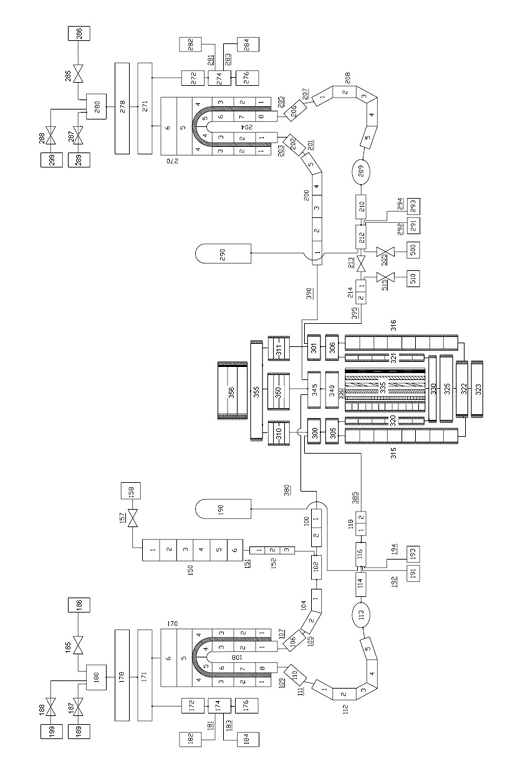
\includegraphics[width=0.85\textwidth]{Images/Nodalization of the Zion NPP.png}
    \caption{RELAP5 nodalization of the Zion Nuclear Power Plant model.}
    \label{fig:ZionNPP_Nodalization}
\end{figure}


\section{Steady State Analysis}
Before starting the accident analysis, it is necessary to verify that the model is in a stable and realistic initial condition.  
A correct steady state is important because the transient results strongly depend on the quality of the initial condition.
The steady-state run is checked by comparing the calculated values with the reference values and by observing the time evolution of the main parameters.  
If the variables remain approximately constant and the deviations from the target values are acceptable, the initial condition can be considered suitable for the transient simulation.
 

                                     

\begin{table}[h]
\centering
\begin{tabular}{lcc}
\toprule
Parameter & Expected value & Steady State Results\\
\midrule
Power (MW) & 3250 & 3250.0\\
Primary pressure in the hot leg (MPa) & 15.5 & 15.5\\
Secondary pressure (MPa) & 6.7 & 6.71\\
Pressurizer level (m) & 8.8 & 8.86\\
Broken Steam Generators DC level (m) & 12.2 & 12.2\\
Intact Steam Generators DC level (m) & 12.2 & 12.2\\
Core outlet temperature (K) & 603 & 603.4\\
Core inlet temperature (K) & 571 & 570.8\\
Broken Main feedwater flow (kg/s) & 459 & 455.8\\
Intact Main feedwater flow (kg/s) & 1325 & 1324.4\\
Intact loop flow (kg/s) & 12865 & 12436\\
Broken loop flow (kg/s) & 4351 & 4356\\
\bottomrule
\end{tabular}
\caption{Expected vs Simulation results for Steady State Values}
\label{tab:Targetvalues}
\end{table}

\tabref{tab:Targetvalues} shows the main variables that must be checked in the steady-state calculation. The steady-state calculation shows that the main plant variables are close to the reference values; small deviations may appear because of nodalization choices, control-system settings, and numerical approximations.  
However, the overall agreement is sufficient to accept the initial condition for the SBO transient analysis.

\subsection{Steady State Verification}
\noindent In this section some plots regarding the steady state case
are provided. The purpose is only to ensure that the calculations done with 
RELAP are coherent with the steady state conditions the plant should be operating at.

\begin{figure}[H]
    \centering
    \begin{minipage}{0.49\textwidth}
        \centering
        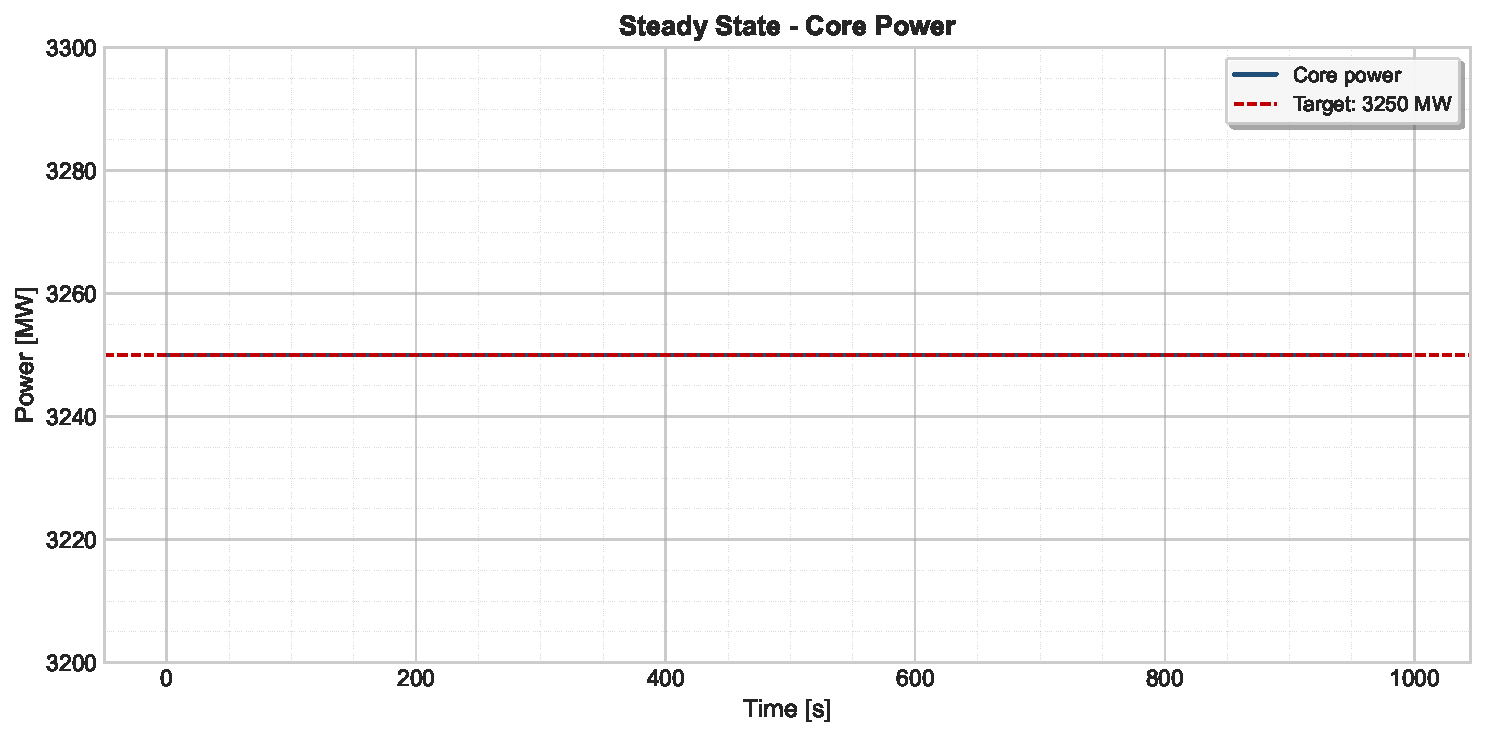
\includegraphics[width=\linewidth]{../Pictures/Steady State/SS1_core_power.pdf}
    \end{minipage}
    \hfill
    \begin{minipage}{0.49\textwidth}  
        \centering
        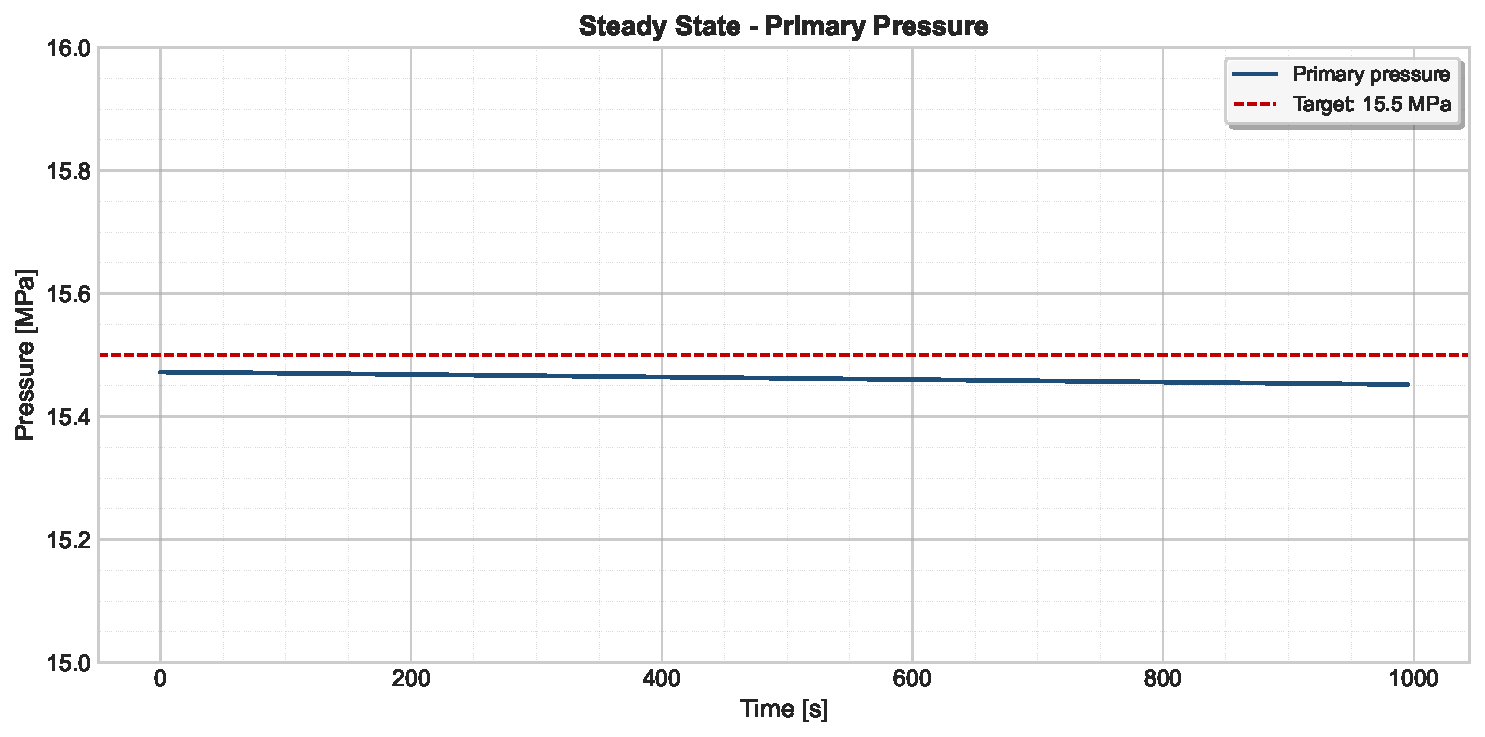
\includegraphics[width=\linewidth]{..//Pictures/Steady State/SS2_primary_pressure.pdf}    
    \end{minipage}
    \caption{\centering {Core Power (on the left) and primary pressure (on the right).}}
    \label{RCS steady}
\end{figure}








\begin{figure}[H]
    \centering
    \begin{minipage}{0.49\textwidth}
        \centering
        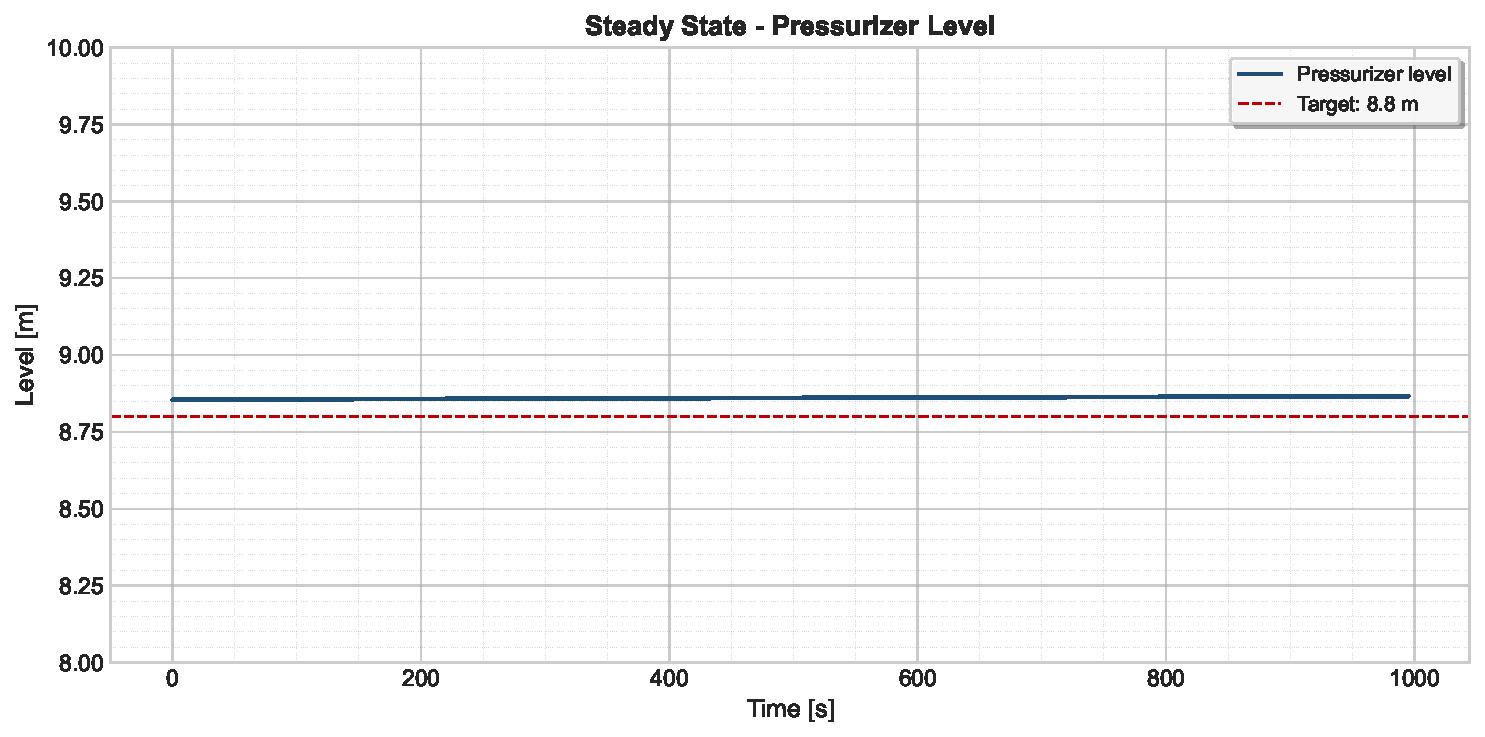
\includegraphics[width=\linewidth]{../Pictures/Steady State/SS4_pressurizer_level.pdf}
    \end{minipage}
    %\hfillSBO FirstReport/Images
    \begin{minipage}{0.49\textwidth}  
        \centering
        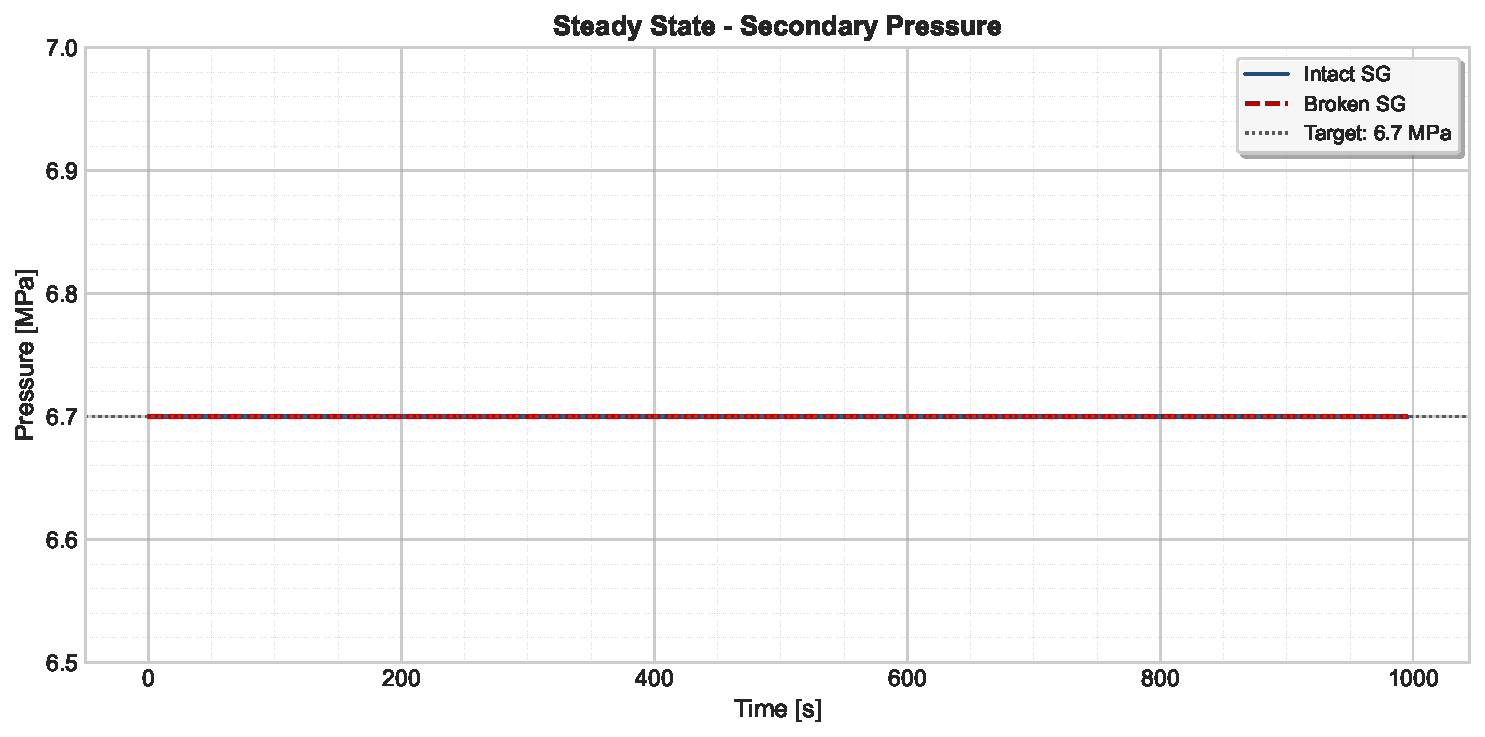
\includegraphics[width=\linewidth]{../Pictures/Steady State/SS3_secondary_pressure.pdf}    
    \end{minipage}
    \caption{\centering {Pressurizer Level (on the left) and Secondary Pressure (on the right).}}
    \label{Presteady}
\end{figure}




\begin{figure}[H]
    \centering
    \begin{minipage}{0.49\textwidth}
        \centering
        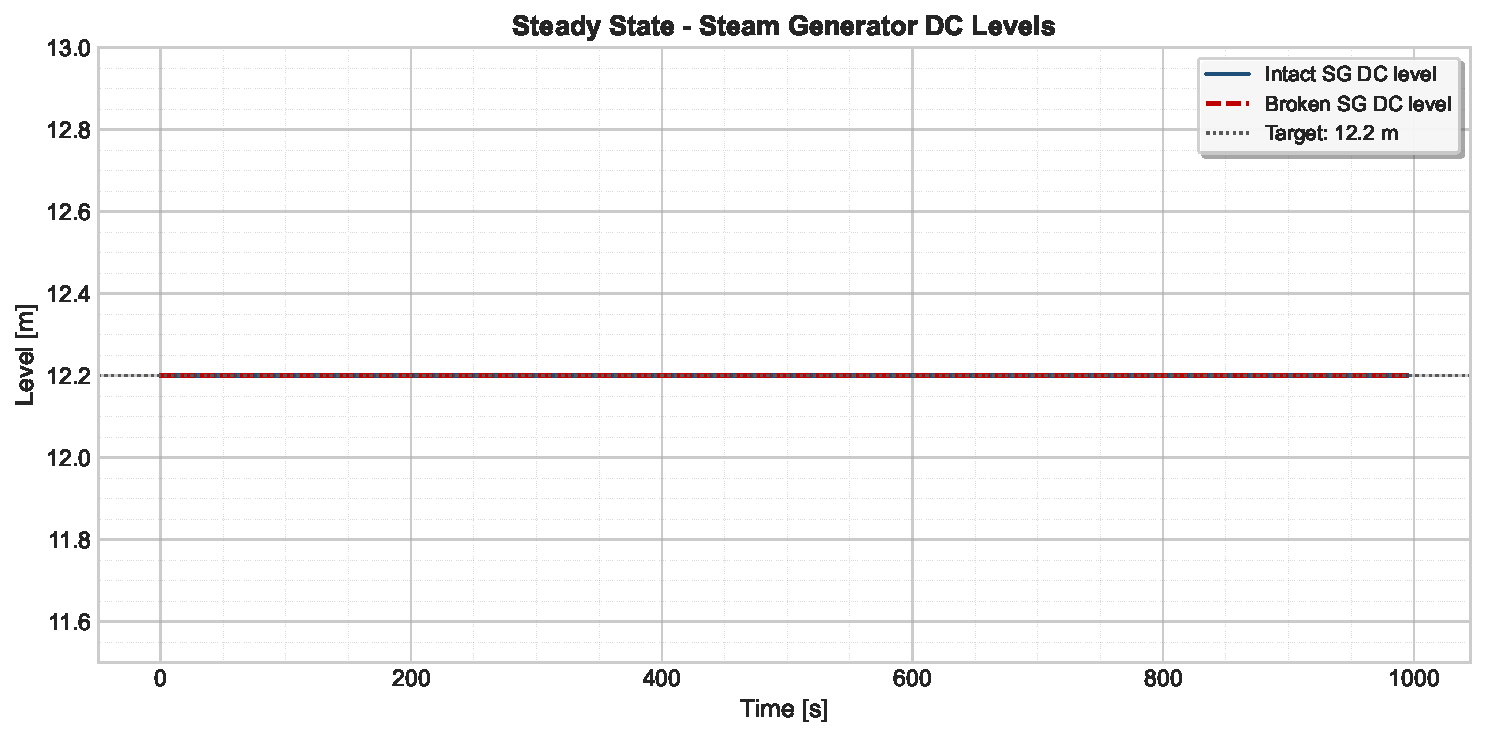
\includegraphics[width=\linewidth]{../Pictures/Steady State/SS5_SG_levels.pdf}
    \end{minipage}
    \hfill
    \begin{minipage}{0.49\textwidth}  
        \centering
        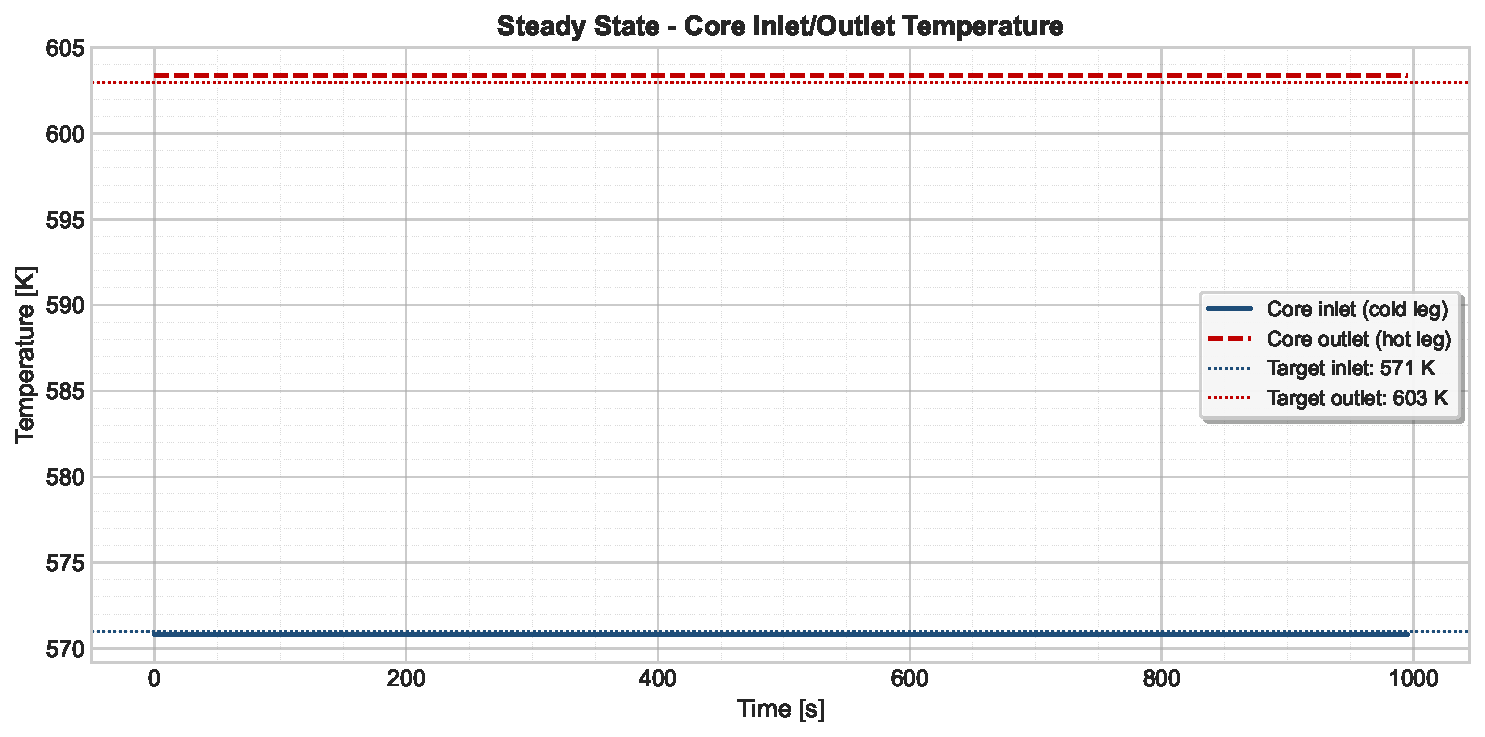
\includegraphics[width=\linewidth]{../Pictures/Steady State/SS6_core_temperatures.pdf}    
    \end{minipage}
    \caption{\centering { SG levels (on the left) and RCS temperatures (on the right).}}
    \label{ss}
\end{figure}


\begin{figure}[H]
    \centering
    \begin{minipage}{0.49\textwidth}
        \centering
        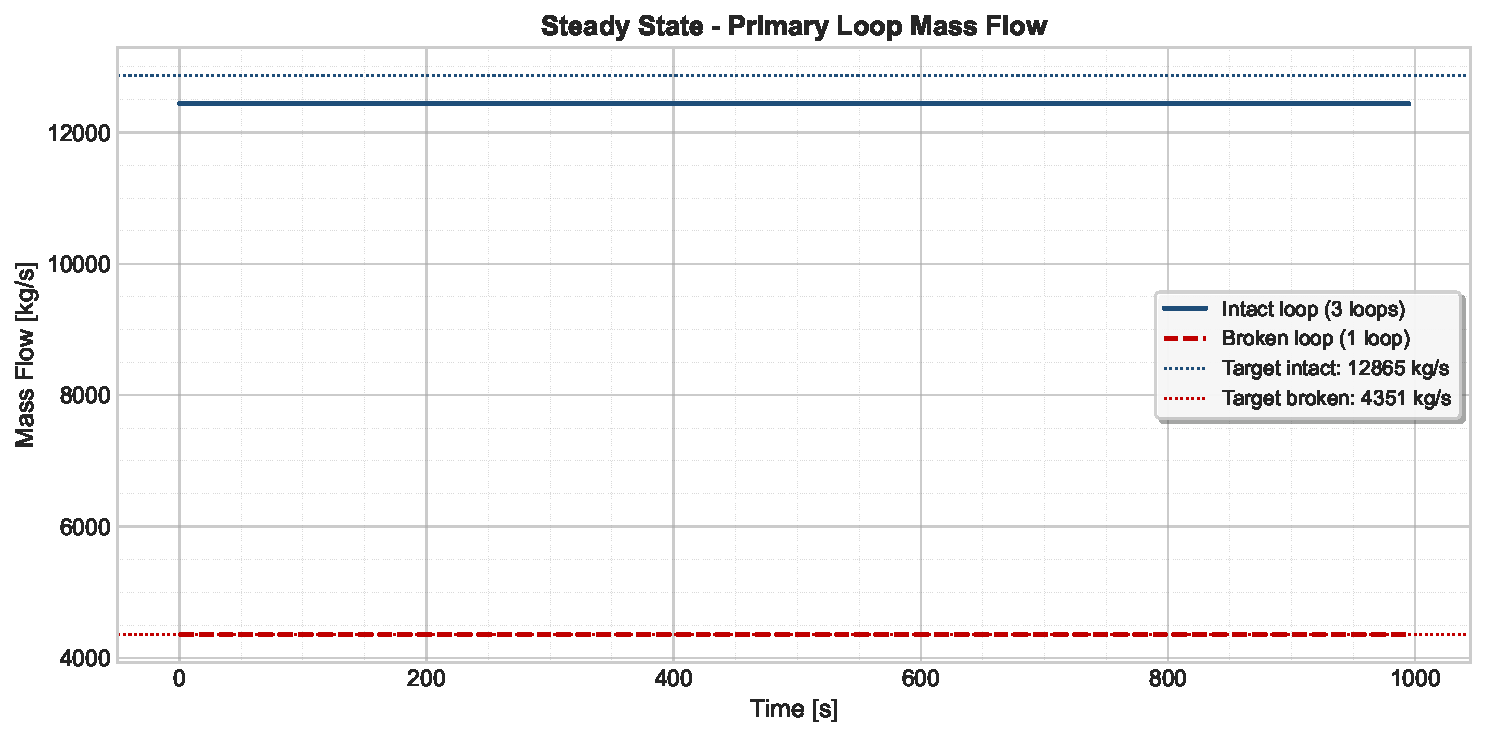
\includegraphics[width=\linewidth]{../Pictures/Steady State/SS7_primary_flow.pdf}
    \end{minipage}
    \hfill
    \begin{minipage}{0.49\textwidth}  
        \centering
        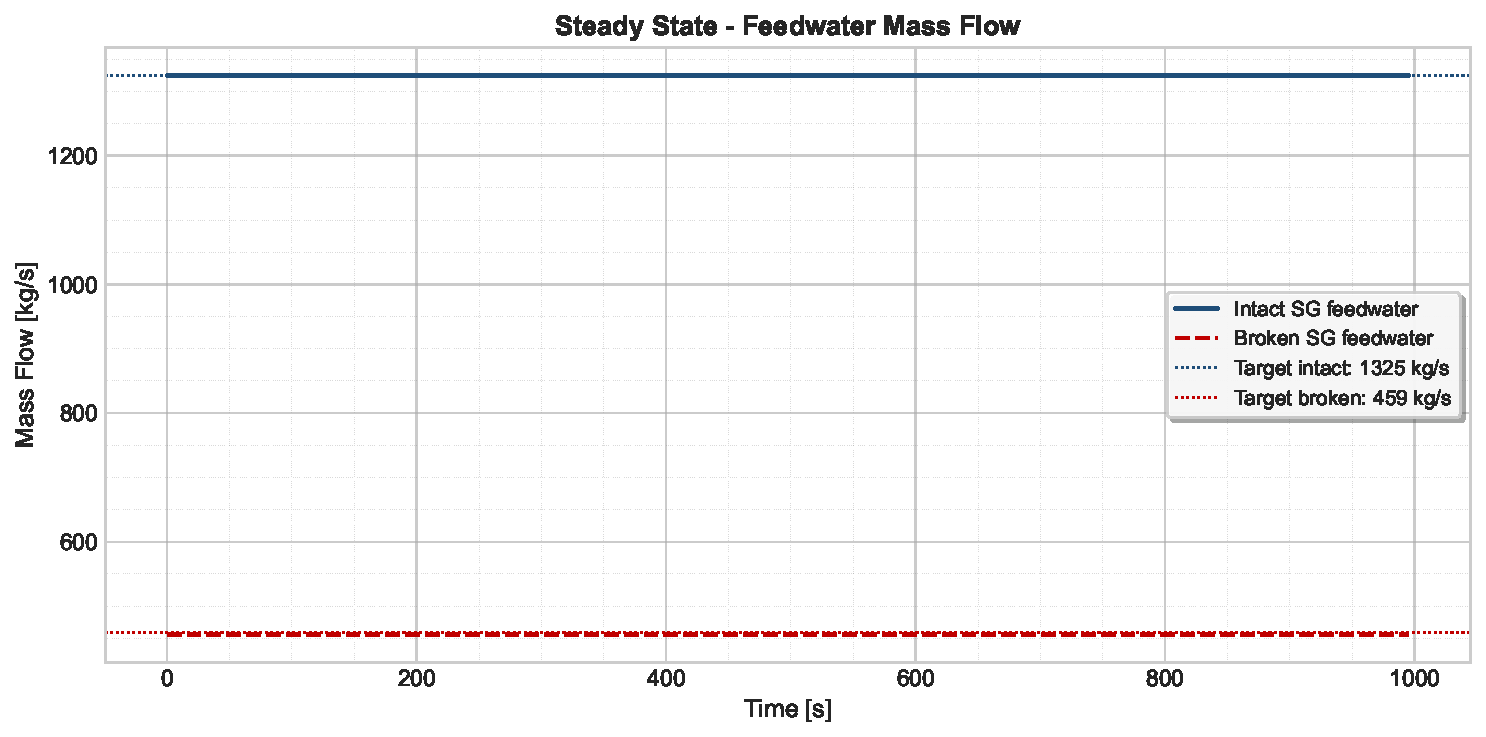
\includegraphics[width=\linewidth]{../Pictures/Steady State/SS8_feedwater_flow.pdf}    
    \end{minipage}
    \caption{\centering {Primary Mass Flow (on the left) and FW Mass Flow (on the right).}}
    \label{flowsteady}
\end{figure}

As we can see, all the variables analyzed are stable and do not change over the time. 
Some of them present little uncertainties that are probably due to numerical errors
and the complexity of the phenomena involved.

\section{Base Case Analysis}

After the steady-state verification, the SBO base case is studied. The Station Black-Out is assumed to begin at $t=0$ s with aggravated conditions. 
Under these conditions, every system that depends on electrical power is considered unavailable. 
As a result, the reactor coolant pumps trip, the control rods are inserted, and other relevant functions, such as the cooling of the pump seals, are lost. 
The general assumptions that are common to all the considered accident sequences are summarized in \tabref{tab:SBO_events} below.

\begin{table}[H]
\centering
\caption{Main events to be included in the SBO base case description.}
\label{tab:SBO_events}
\begin{tabular}{p{4.5cm} p{10.5cm}}
\toprule
\textbf{Event / action} & \textbf{Short description} \\
\midrule
SBO initiation & Loss of off-site and on-site AC power according to project assumptions \\
Reactor scram & Automatic shutdown following the transient logic \\
RCP trip & Reactor coolant pumps stop after loss of power \\
FW / AFW behavior & Feedwater and auxiliary feedwater response according to the base-case logic \\
Pressurizer systems & Heater and control-system behavior during SBO \\
Safety injection unavailability & HPSI and LPSI unavailable during the transient \\
Steam line / relief actions & Valve actions according to the project assumptions \\
Additional operator actions & To be completed based on the adopted base-case procedure \\
\bottomrule
\end{tabular}
\end{table}

In order to simulate all the accidental sequence, some actions that 
could be performed from the operators have been taken into account. These are
listed below. 








\begin{table}[h!]
\centering
\renewcommand{\arraystretch}{1.3}
\begin{tabular}{|p{4.5cm}|p{10.5cm}|}
\hline
\textbf{Action / Event} & \textbf{Description} \\ \hline
RCP Seal Leak & Starts 10 minutes after SBO initiation with a leak size of 0.00001 m2 per pump. \\ \hline
Leak area increase & The leak area increases 4x when saturation takes place at the RCP. \\ \hline
TDP AFW Injection & Auxiliary feed water is provided by a turbo-driven pump (TDP) which is controlled manually and requires batteries. \\ \hline
TDP battery depletion & Batteries last for 5h, after which the TDP becomes uncontrolled, injecting water until the separator is flooded and the TDP stops. \\ \hline
Cooldown strategy (EOP) & Operators follow a strategy to cool down the SG at a rate of 55 K/h until 15 bar. \\ \hline
Primary depressurization (EOP) & Operators fully open the Pressurizer relief valves to depressurize the primary system if the Core Exit Temperature is higher than 923 K. \\ \hline
AC power recovery & Recovery of AC power occurs after 12h, which recovers AFW, HPIS, and LPIS. \\ \hline
\end{tabular}
\caption{Configurable actions and conditions for the SBO sequences in the Zion model}
\label{tab:sbo_actions_en}
\end{table}

\subsection{First Analysis}

\noindent The first analysis was performed considering that all the EOPs
listed in \tabref{tab:sbo_actions_en} have taken place. We are going to 
analyze the transient in order to verify the situation of the plant after the 
SBO has occurred. 

\subsubsection{Reactor Coolant System}

\noindent Right after the SBO event, the SCRAM immediately shuts down 
the reactor by inserting the control rods, leading to a rapid decrease in power, that 
is plotted in \figref{power}. The residual value present in the graph 
is due to the decay heat, which represents the main issue in this types of scenarios.
Moreover, the loss of AC power causes the immediate trip of the pumps.

\begin{figure}[H]
    \centering
    \begin{minipage}{0.49\textwidth}
        \centering
        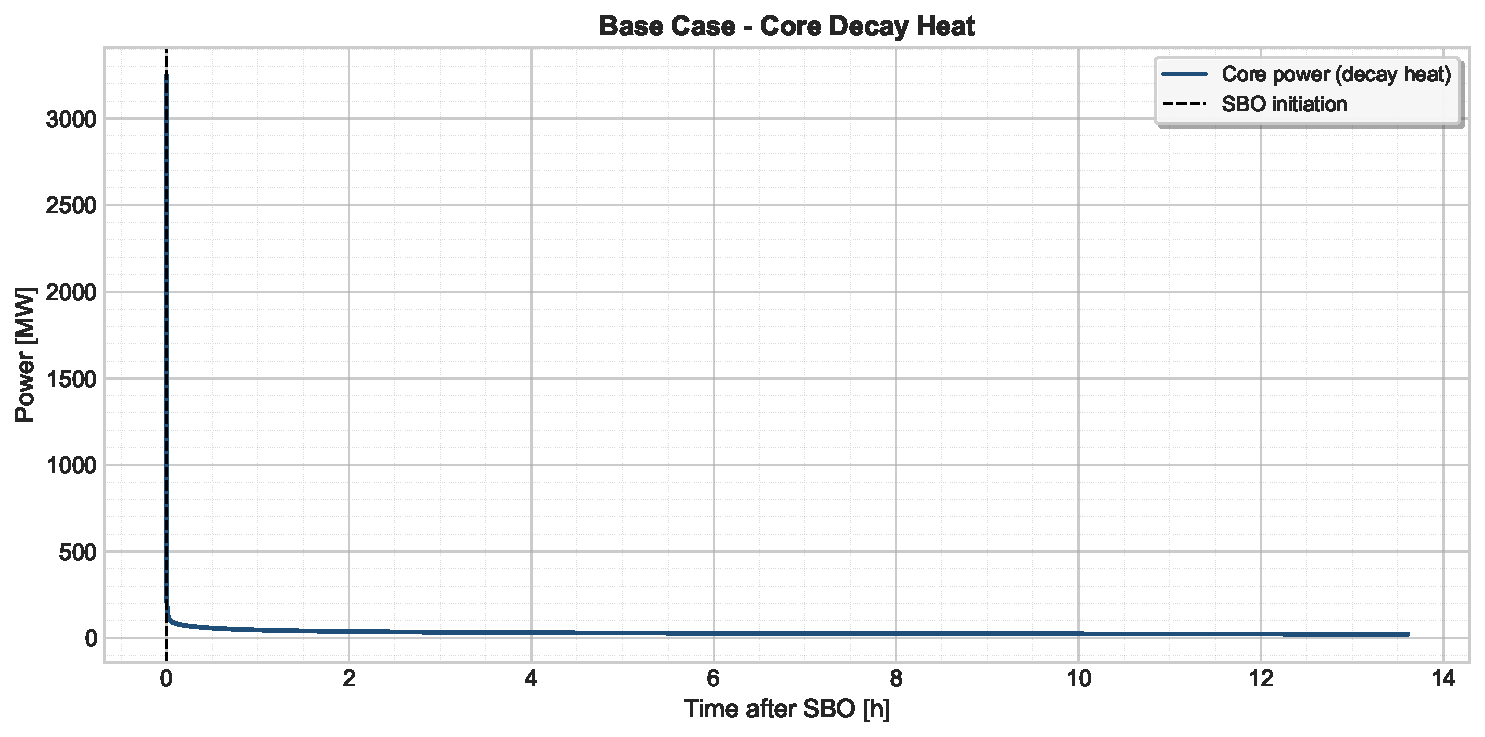
\includegraphics[width=\linewidth]{../Pictures/Base Case/BC1_core_power.pdf}
    \end{minipage}
    \hfill
    \begin{minipage}{0.49\textwidth}  
        \centering
        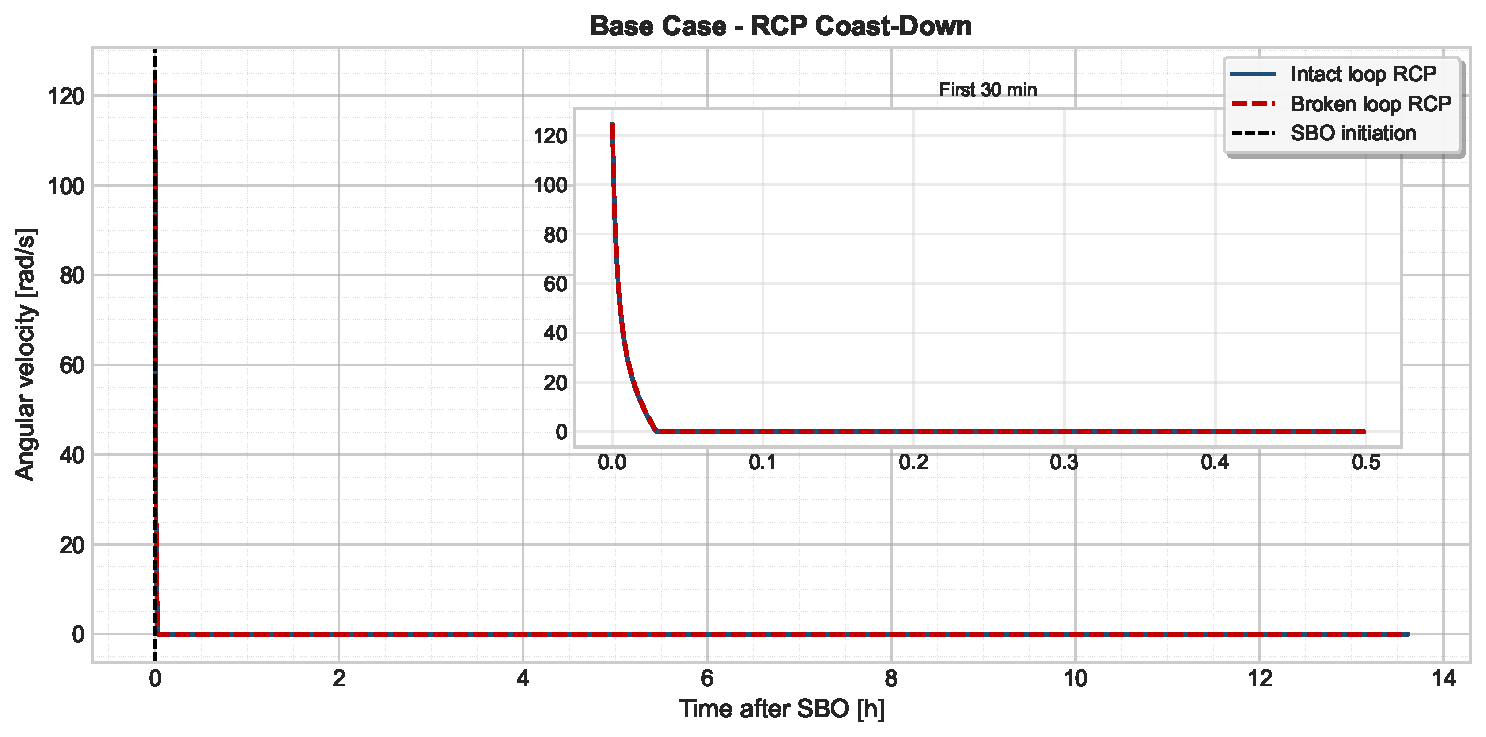
\includegraphics[width=\linewidth]{../Pictures/Base Case/BC7_RCP_velocities.pdf}    
    \end{minipage}
    \caption{\centering {Core Power (on the left) and RCP velocities (on the right).}}
    \label{power}
\end{figure}



\noindent The sudden power decrease causes a contraction within the coolant, 
which lowers the level inside the pressurizer, as it is shown in \figref{plevels}.
The level reaches zero and it starts to increase again after 12 hours, when 
the AC power is recovered and water is introduced again by the means of HPIS, LPIS and the pumps. The loss of level is also enhanced by the loss of inventory, as 
the seal injection system is not available during a SBO. This lead to some leaks from the pumps, which contributes to the decrease.
However, an empty pressurizer does not imply that the core is uncovered. This situation 
is properly described in \figref{plevels}.

\begin{figure}[H]
    \centering
    \begin{minipage}{0.49\textwidth}
        \centering
        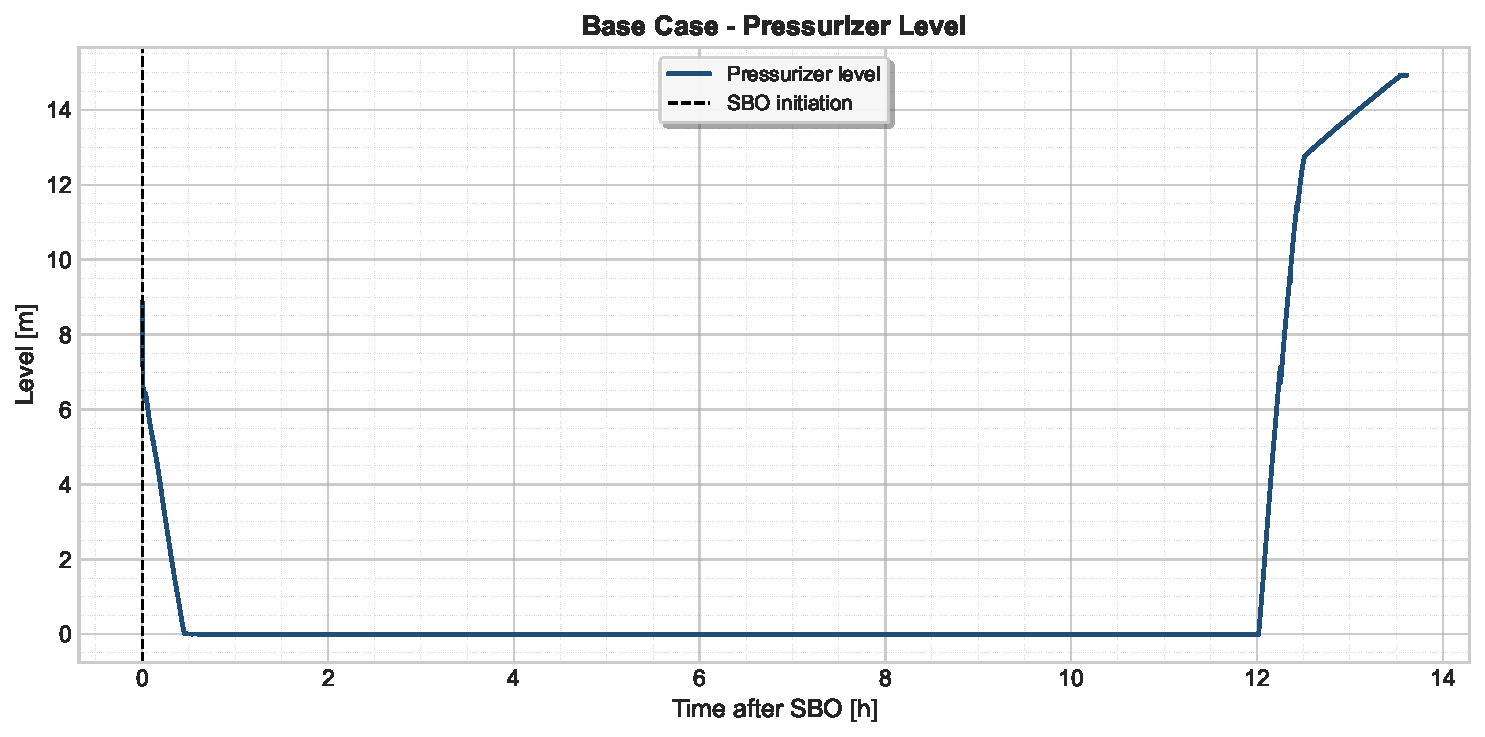
\includegraphics[width=\linewidth]{../Pictures/Base Case/BC4_pressurizer_level.pdf}
    \end{minipage}
    \hfill
    \begin{minipage}{0.49\textwidth}  
        \centering
        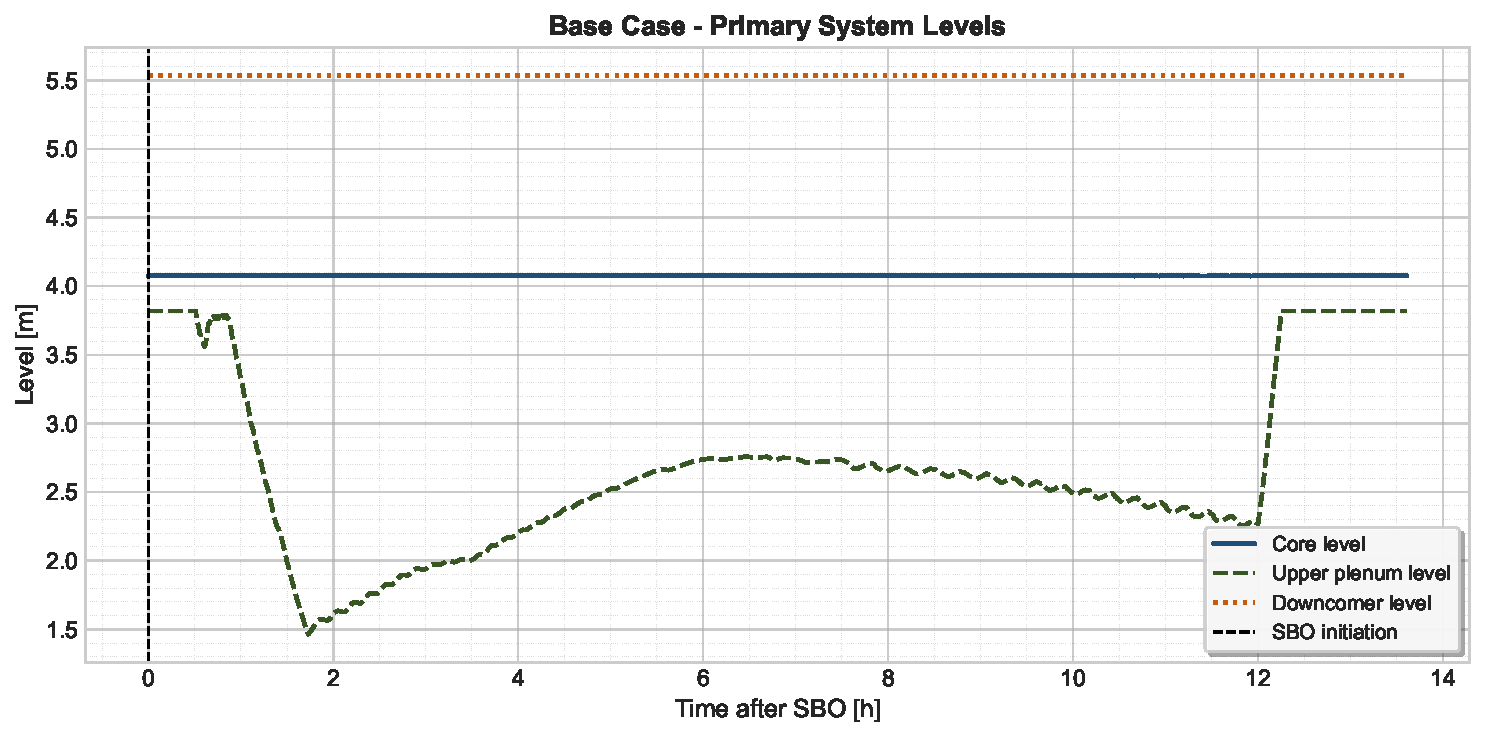
\includegraphics[width=\linewidth]{../Pictures/Base Case/BC6_primary_levels.pdf}    
    \end{minipage}
    \caption{\centering {Pressurizer Level (on the left) and Core Levels (on the right).}}
    \label{plevels}
\end{figure}




In \figref{RCP} the pumps's leaks is shown. 


\begin{figure}[H]
    \centering
    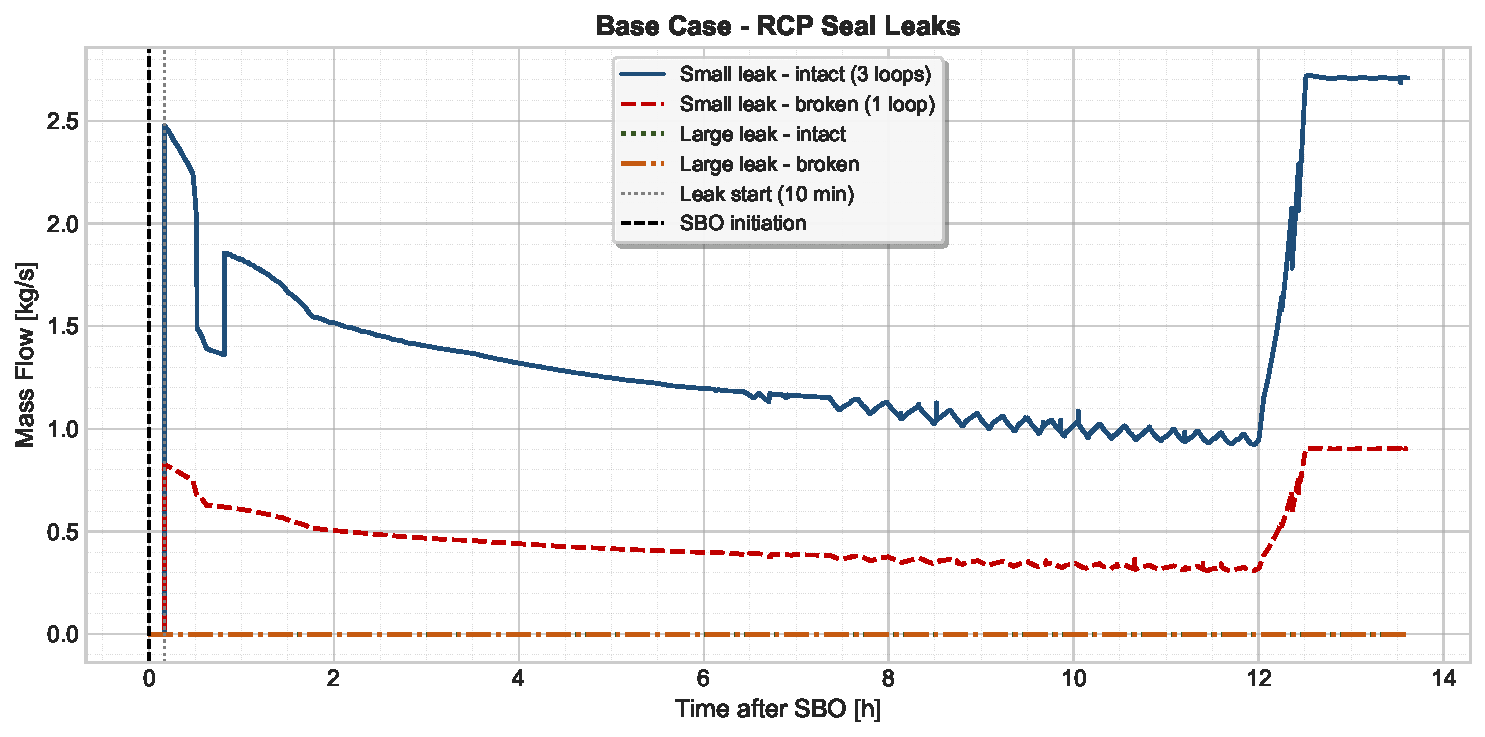
\includegraphics[width=0.55\linewidth]{../Pictures/Base Case/BC12_RCP_seal_leaks.pdf}
    \caption{\centering RCP Seals Leaks. Notice that the intact loop represents 3 loops.}
    \label{RCP}
\end{figure}

According to the EOPs, if the outlet temperature from the core is higher than 
923 K, the operators should depressurize the primary system using the PRZ valves. In our case, this procedure
has not been necessary, as the core exit temperature does not overcome 923 K. \figref{tprimary} shows the main parameters related to 
the temperatures of the core.


\begin{figure}[H]
    \centering
    \begin{minipage}{0.49\textwidth}
        \centering
        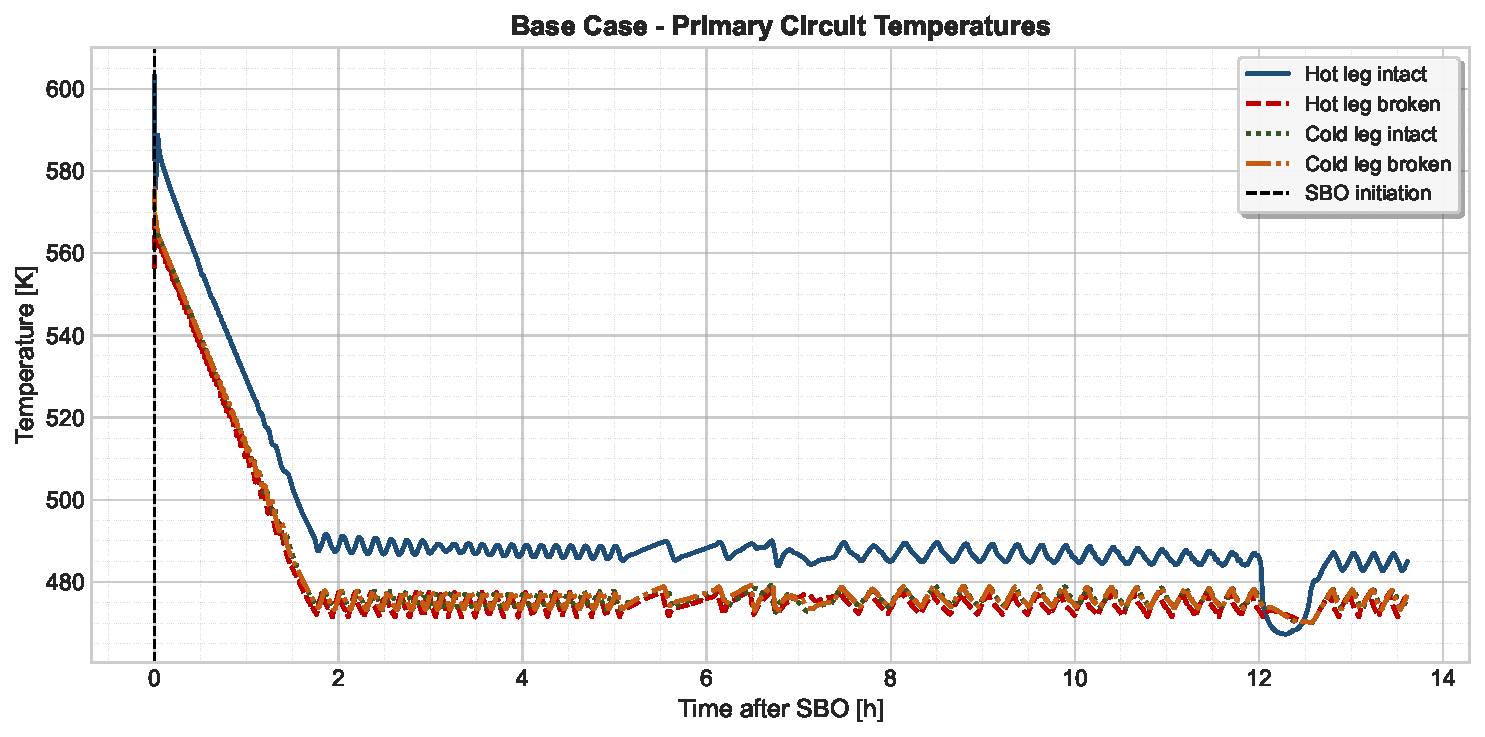
\includegraphics[width=\linewidth]{../Pictures/Base Case/BC8_primary_temperatures.pdf}
    \end{minipage}
    \hfill
    \begin{minipage}{0.49\textwidth}  
        \centering
        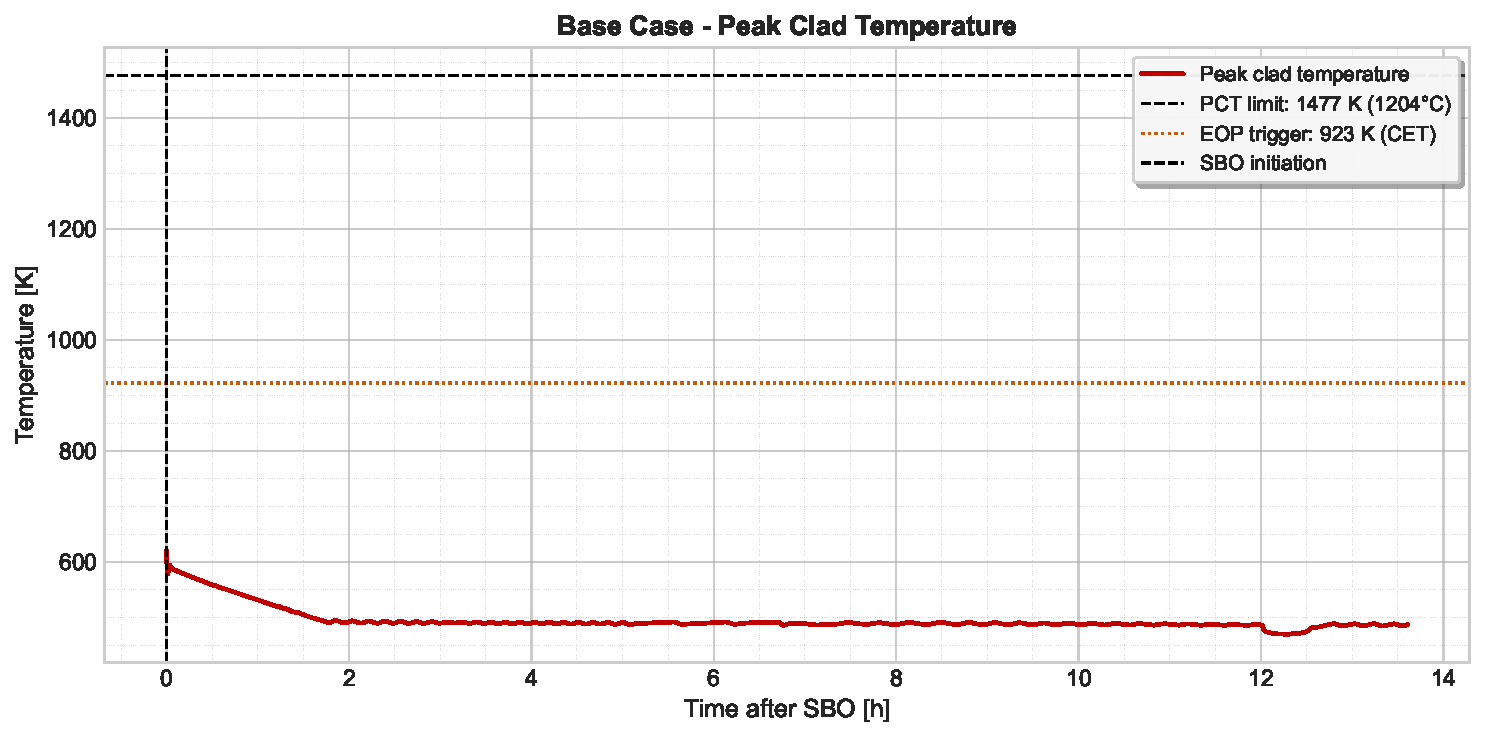
\includegraphics[width=\linewidth]{../Pictures/Base Case/BC10_peak_clad_temperature.pdf}    
    \end{minipage}
    \caption{\centering {Core Temperatures (on the left) and Cladding Temperature (on the right).}}
    \label{tprimary}
\end{figure}

The primary temperatures are lower than the threshold limit established 
for the operator, as well as the peak cladding temperature. It remains lower than the safety limit, preventing 
damages to the cladding. It also indicates that DNBR is prevented and the core is covered. The constant behaviour can be explained 
as a consequence of some natural circulation phenomena that could have taken place inside the primary, due to the pressure difference 
between primary and secondary. \figref{flow} shows that a little flow inside the RCS 
is present, even if the pumps are tripped. The natural circulation guarantees the heat exchange 
between the core and the SGs.


\begin{figure}[H]
    \centering
    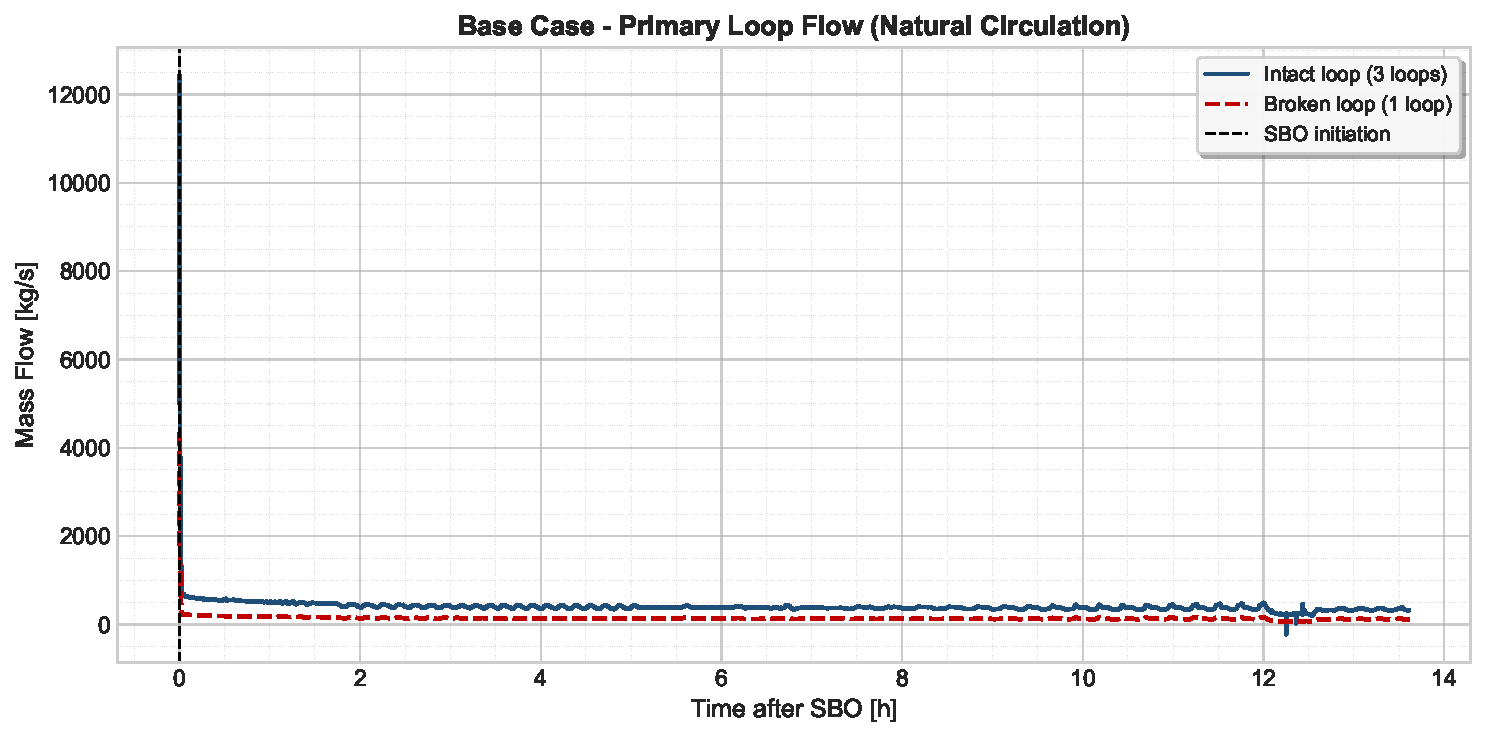
\includegraphics[width=0.55\linewidth]{../Pictures/Base Case/BC15_primary_flow.pdf}
    \caption{\centering Primary Mass Flow}
    \label{flow}
\end{figure}

\subsection{Secondary System}
\noindent It is finally the moment to take a look at the behaviour 
of the secondary system. In a SBO scenario, this system plays a fundamental role, since 
it is used to extract the heat coming from the core where no AC powered system is available. A natural circulation
flow regime is established by the pressure's difference between the primary and the secondary, helped by the elevation of the latter. In fact, 
the SG is usually located in a higher position than the core, in order to stimulate
the gravity forces that act by density. \\
As we said in the previous chapter, a cooldown procedure is performed by the operators. The aim is to 
cool down the SG at a rate of 55 K/h, until a pressure of 15 bar (1.5 MPa)
within the secondary is guaranteed. In \figref{sgp} this situation is well 
described.

\begin{figure}[H]
    \centering
    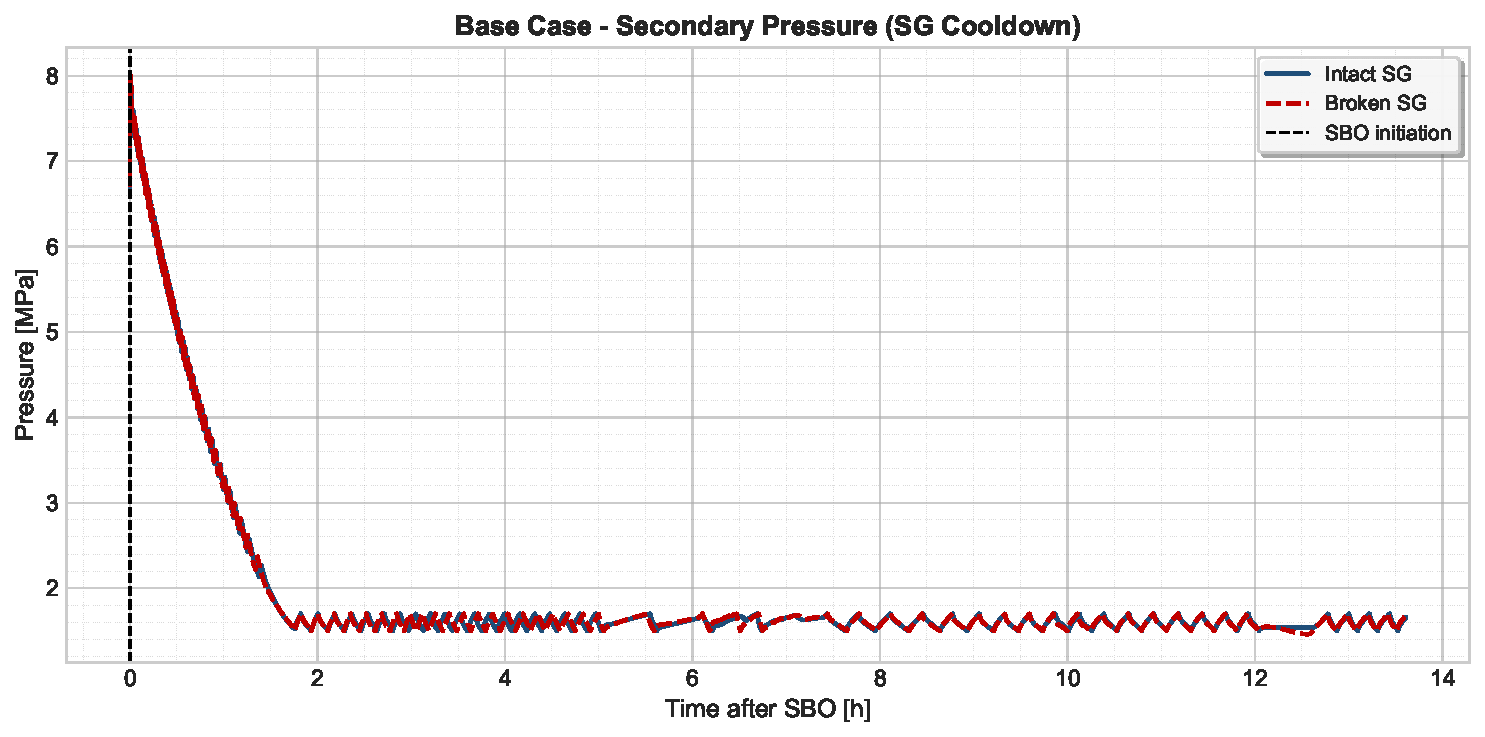
\includegraphics[width=0.55\linewidth]{../Pictures/Base Case/BC3_secondary_pressure.pdf}
    \caption{\centering SG Pressure Evolution during the Transient.}
    \label{sgp}
\end{figure}
The procedure is done by the relief valves, located at the top of the SG. Their function is to release steam to the atmosphere, 
in order to reduce the pressure inside the SG. As we can see from the picture, 
the procedure is well carried out until the target pressure of 15 bar is reached. 



\begin{figure}[H]
    \centering
    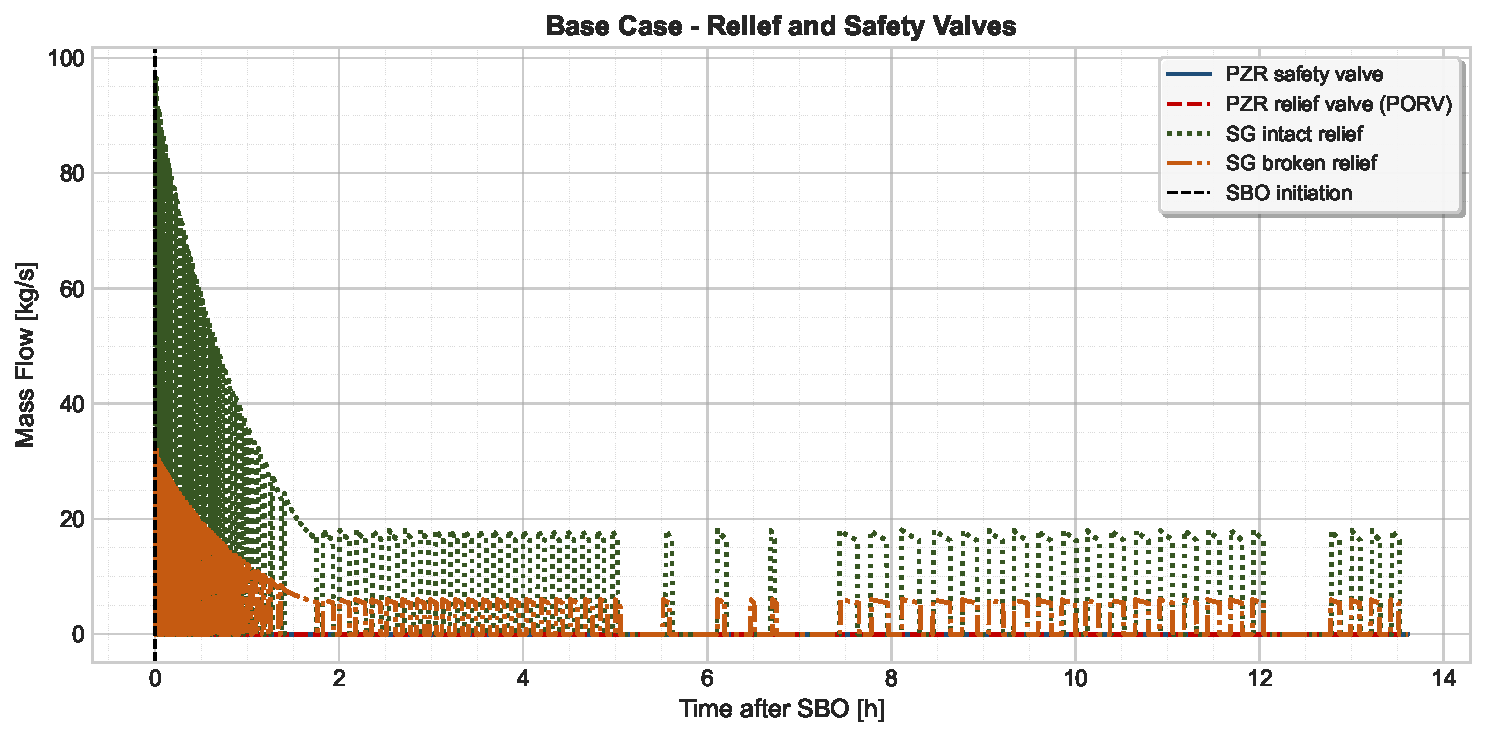
\includegraphics[width=0.55\linewidth]{../Pictures/Base Case/BC13_relief_valves.pdf}
    \caption{\centering Relief Valves Flow. Notice that the flow coming from the PRZ valves is zero, as the primary depressurization has not been carried.}
    \label{relief}
\end{figure}

\figref{relief} shows the flows coming from the relief valves. The behaviour of the valves is coherent with 
the SG pressure curve, the most of the steam is released at the beginning of the procedure and gradually decreases. After that, 
the flow remains constant, since the operators aimed to keep the SG pressure constant and the Auxiliary FeedWater is constantly injecting 
water. The latter is shown in \figref{AFW1}. The batteries that power the turbo-driven AFW last for 5 hours. As mentioned in \tabref{tab:sbo_actions_en}, at this moment 
the TDP becomes uncontrolled and injects water until the SG separator is flooded. 

\begin{figure}[H]
    \centering
    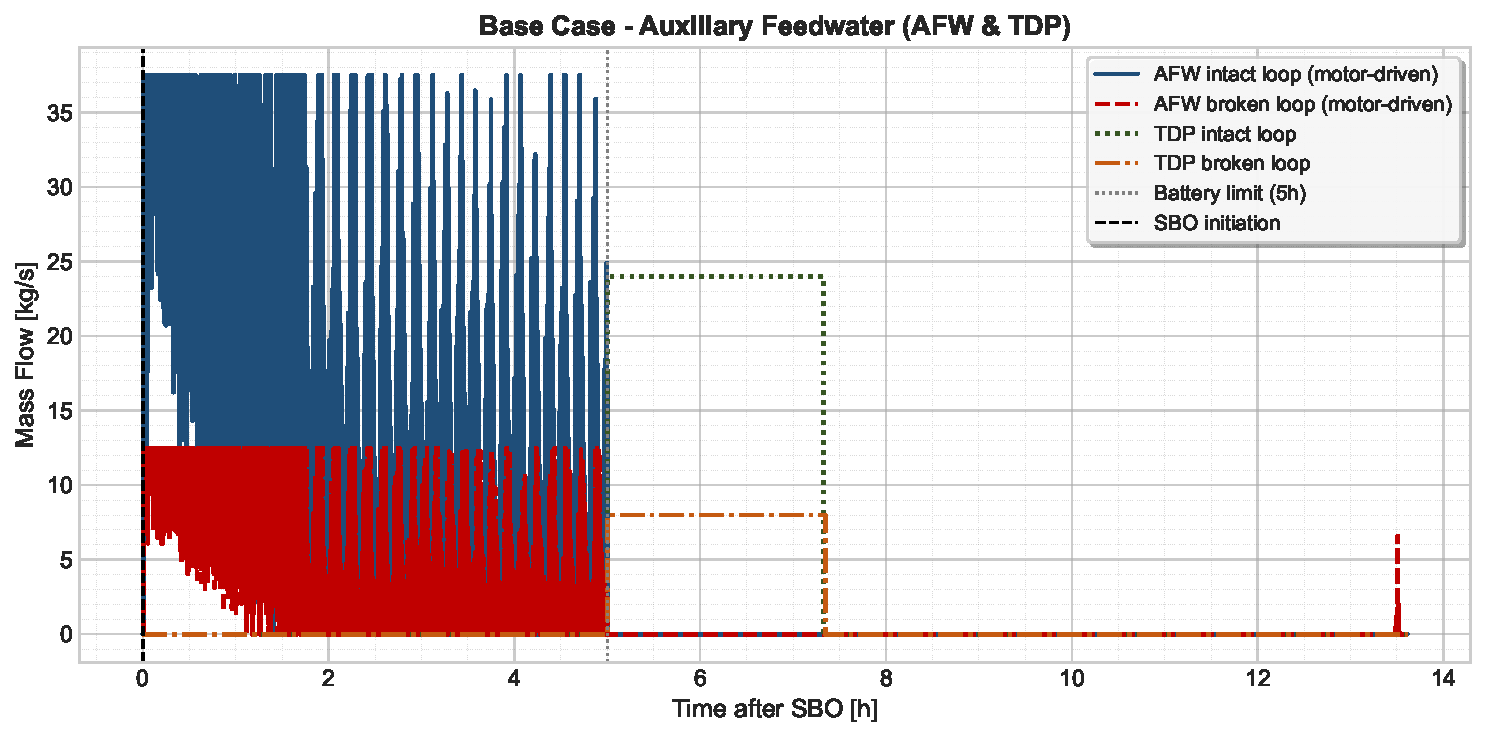
\includegraphics[width=0.55\linewidth]{../Pictures/Base Case/BC11_AFW_TDP.pdf}
    \caption{\centering Auxiliary Turbo-Driven Feedwater Flow. Remember that the intact loop represents 3 loops. }
    \label{AFW1}
\end{figure}


\section{Additional Calculations}
\noindent As part of the base case simulation, there are two operator procedures assumed to be preformed. These are the steady depressurization of the secondary system, and the depressurization of the primary based on a high outlet core temperature. 
Apart from the complete base case, the simulation was also performed without these operator interventions in order to gauge their effectiveness. The second EOP mentioned above, pertaining to primary depressurization, was never actuated in the base case as the outlet temperature never reached the threshold value. Therefore, this case was identical to the base case and will not be analyzed further and only the additional case without the EOP 1  is analyzed below. This simulation analyzes the dynamics and critical values of the system when the steam generators are not depressurized allowing for a further reduction in primary temperature and pressure. 

\figref{PSNOSG} below demonstrates the lack of pressure relief of the secondary system. The lack of the depressurization EOP maintains the pressure high in the secondary system. This graph verifies that the EOP is not initiated as intended. In the base case, the relief valve setpoint is progressively reduced from the nominal value of 6.7 MPa down to 1.5 MPa, following the 55 K/h cooldown ramp. Without this operator action, the setpoint remains fixed at the nominal opening value of 7.58 MPa throughout the entire transient. As a consequence, the secondary pressure does not decrease monotonically but instead exhibits a strong cyclic behaviour: as the decay heat continuously produces steam, the pressure rises until the relief valve opens at 7.58 MPa, releasing steam to the atmosphere. Once the pressure drops below the closing setpoint of 7.79 MPa, the valve closes and the pressure begins to rise again. This open-close cycling of the relief valves repeats continuously, maintaining the secondary pressure oscillating between approximately 4.5 and 8.0 MPa rather than reaching the 1.5 MPa target of the EOP.
%Graph of Secondary Pressure


\begin{figure}[H]
    \centering
    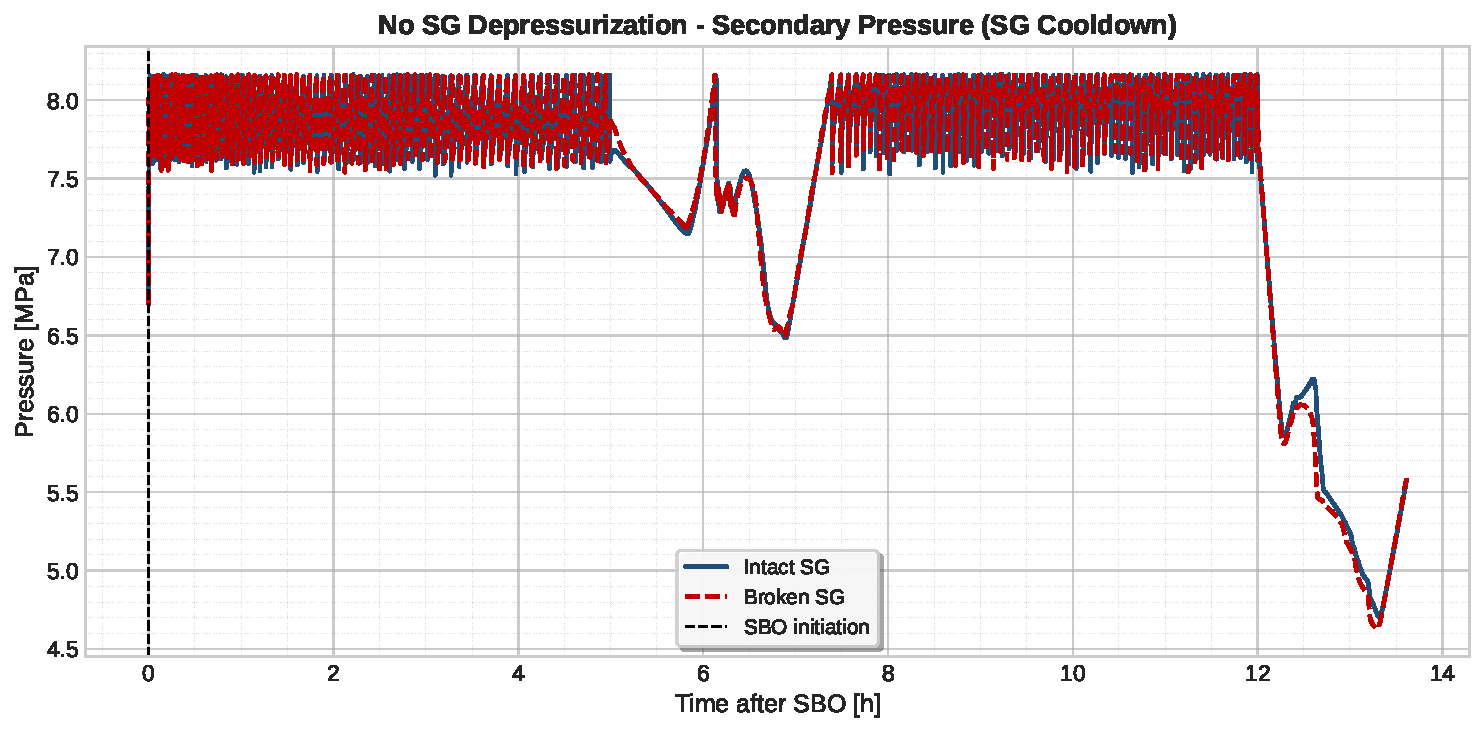
\includegraphics[width=0.55\linewidth]{../Pictures/No SG Case/noSG3_secondary_pressure.pdf}
    \caption{\centering Secondary Pressure. }
    \label{PSNOSG}
\end{figure}




One of the main concerns during the transient event is the protection of the fuel cladding. \figref{TcladNOSG} shows the temperature of the cladding as a way to verify a lack of oxidation of the zirconium. The temperature in the primary does not reach excessive levels. Although it is higher than the base case which sees a drop in temperature of the cladding shortly after the event initiation, the temperature is still a safe margin away from rapid oxidation.

\begin{figure}[H]
    \centering
    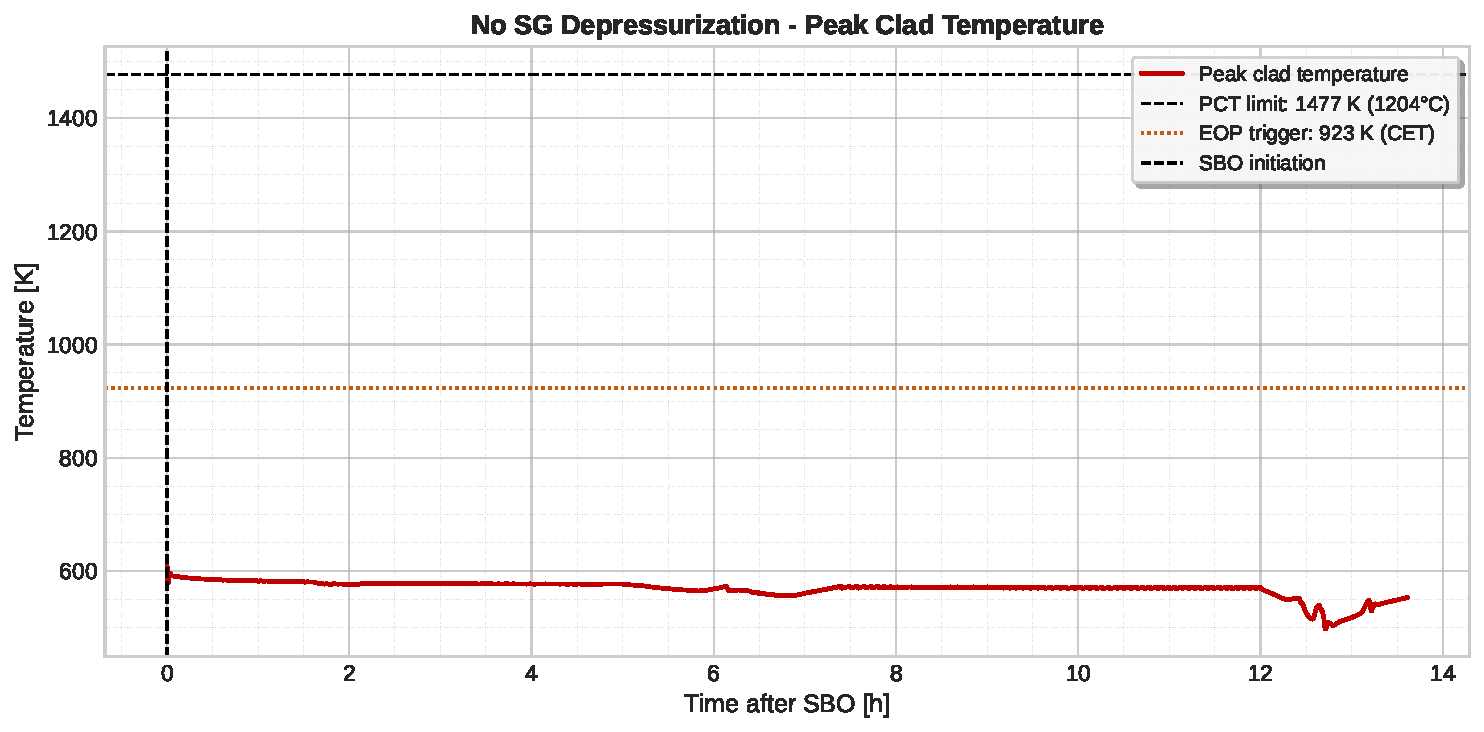
\includegraphics[width=0.55\linewidth]{../Pictures/No SG Case/noSG10_peak_clad_temperature.pdf}
    \caption{\centering Peak Cladding Temperature.}
    \label{TcladNOSG}
\end{figure}


Another factor of concern is the pressure in the primary. Without the further cooldown of primary system as a result of the steam generator depressurization, the pressure in the primary is much more elevated. One of the main concerns of this value is the correlation between leak rate and pressure. With higher primary pressures, we can expect to lose more inventory through the RCP seals.
This situation is well represented in \figref{primaryNoSG}.

\begin{figure}[H]
    \centering
    \begin{minipage}{0.49\textwidth}
        \centering
        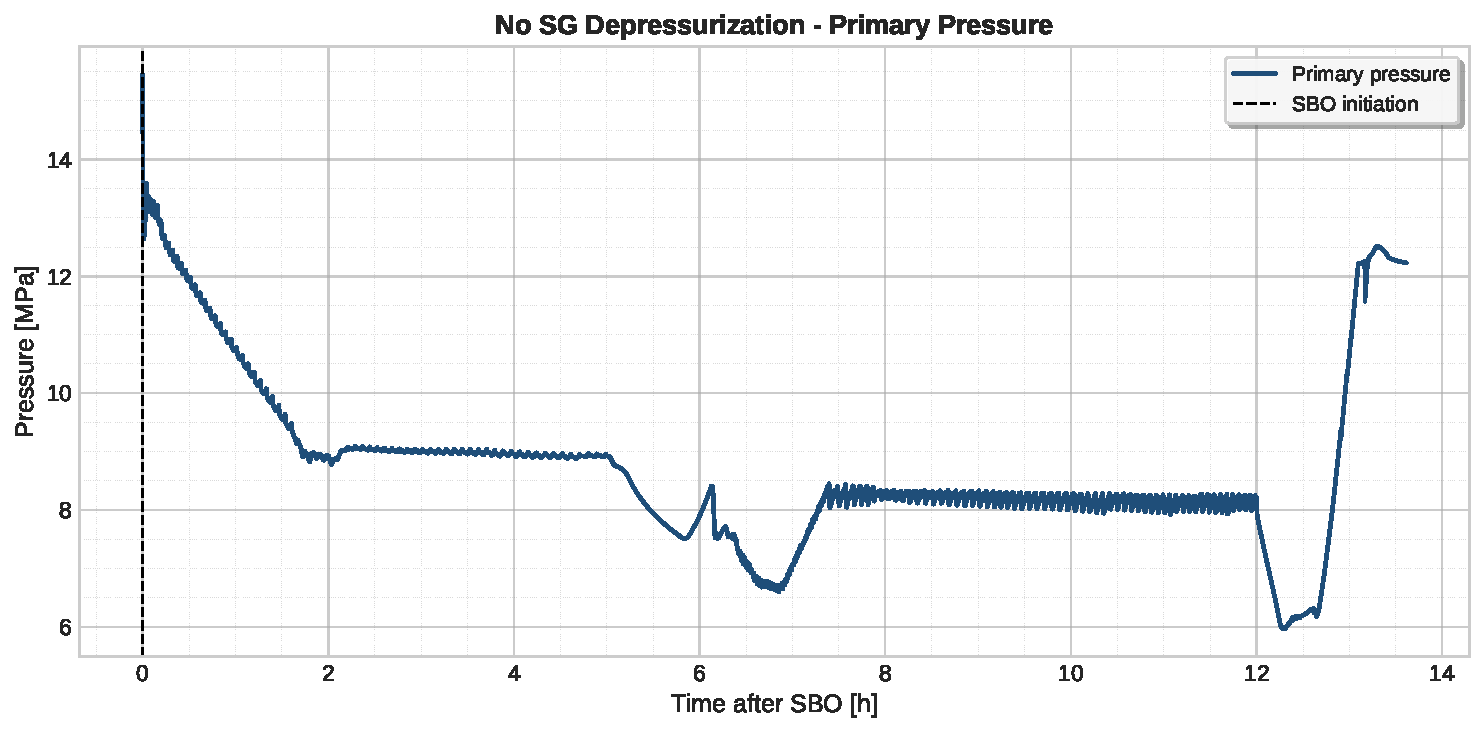
\includegraphics[width=\linewidth]{../Pictures/No SG Case/noSG2_primary_pressure.pdf}
    \end{minipage}
    \hfill
    \begin{minipage}{0.49\textwidth}  
        \centering
        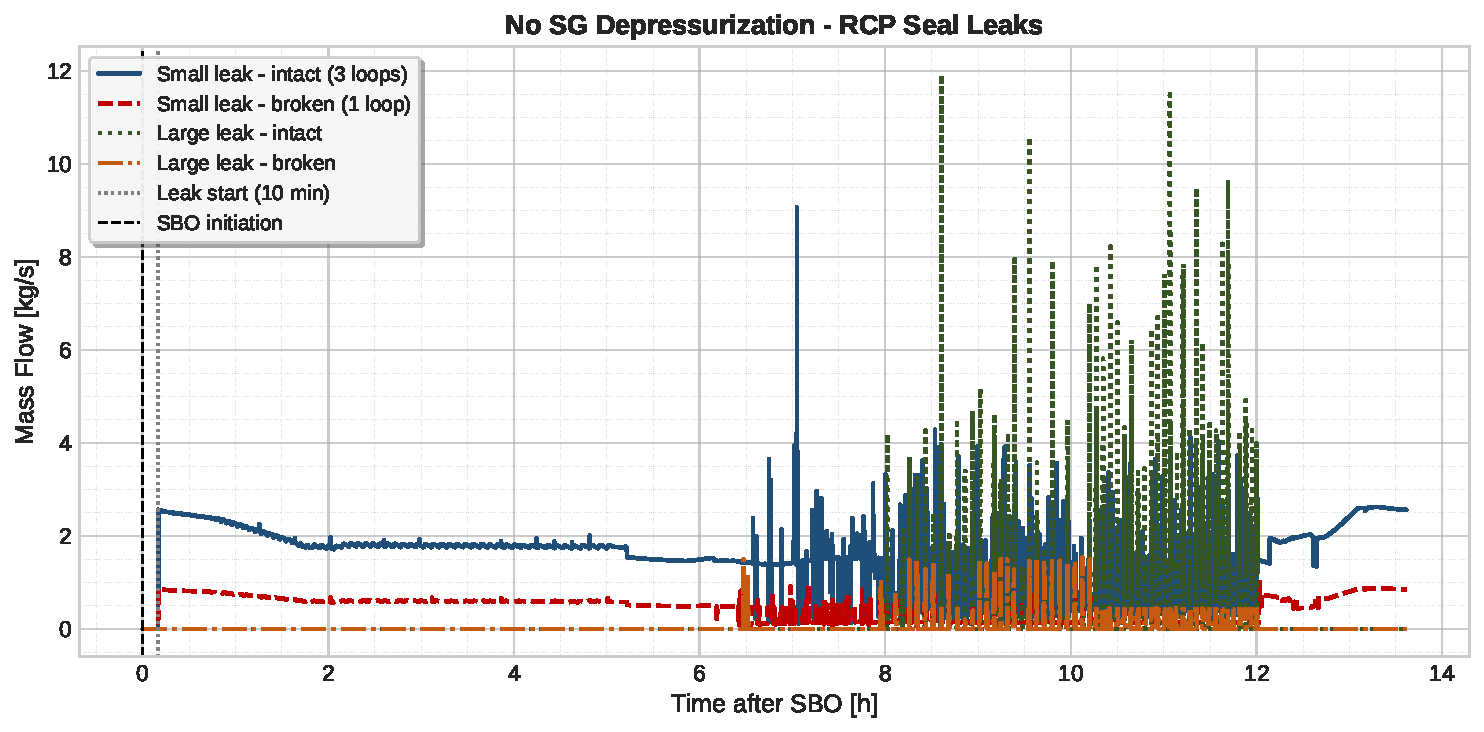
\includegraphics[width=\linewidth]{../Pictures/No SG Case/noSG12_RCP_seal_leaks.pdf}    
    \end{minipage}
    \caption{\centering {Primary pressure (on the left) and RCP seal leak rate (on the right).}}
    \label{primaryNoSG}
\end{figure}

As discussed above, the leak rate of the RCP seals is of concern in this event, and becomes more of an issue with higher primary pressures. \figref{primaryNoSG} confirms this. The higher primary pressure has a direct consequence on the RCP seal leak rates. Since the leak flow is driven by the pressure difference between the primary circuit and the containment atmosphere, a higher primary pressure results in a significantly larger leak flow. The seal leak rates in the no-cooldown case reach peak values of approximately 8-10 kg/s for the intact loop, compared to roughly 2.5 kg/s in the base case — about 3-4 higher. The irregular oscillating pattern of the leak rate directly correlates with the cyclic pressure oscillations of the secondary system described above. Despite this increased inventory loss, no core uncovery is observed within the 12-hour simulation window, indicating that the plant remains in a safe condition. However, in a longer SBO scenario, the sustained high leak rate would represent a more serious concern for primary inventory management.

The simulation demonstrated that the EOP does help to reduce the temperature of the core and the pressure of the primary system. However, based on this analysis is not essential in order to protect the integrity of the fuel cladding during a 12 hour station black out. 

\newpage 
\section{Event tree for the SBO scenario}
The event Tree analysis is an inductive procedure that aims to show all the possible outcomes of an initiating event, in our case an SBO with aggravated conditions. The objective is to identify all the potential accident scenario in a complex frequency. At the end of the process, it is possible to calculate the core damage frequency by assigning a frequency to each sequence. In this part an event tree for the SBO scenario regarding the ZION nuclear power plant is presented, together with the PSA frequency calculation. 

\subsection{Initiating Event and Top Events considered in this analysis}

The initiating event is the SBO occured in aggravated conditions. It implies that all the systems that require power are unavailable. The top events that were chosen to be analyzed in this event tree are listed in \tabref{TOPEVENTS}. 

\begin{table}[H]
\centering
\caption{Top events considered in the SBO event tree.}
\label{tab:top_events}
\renewcommand{\arraystretch}{1.25}
\begin{tabular}{@{}cl>{\raggedright\arraybackslash}p{4.6cm}c>{\raggedright\arraybackslash}p{3.6cm}@{}}
\toprule
\textbf{ID} & \textbf{Top event} & \textbf{Description} & \textbf{Timing} & \textbf{Success criterion} \\
\midrule
TE1 & Small leak &
RCP seal LOCA induced by loss of seal injection and thermal barrier cooling. Break area $1\times 10^{-5}\ \mathrm{m^2}$ per pump (intact loop counts as three pumps). &
$t = 10$ min &
Seal integrity maintained; no leak develops. \\

TE2 & AFW \& TDP &
Turbine-driven pump delivers auxiliary feedwater to the steam generators, providing the only available secondary heat sink during SBO. &
$t = 0^{+}$ (on demand) &
TDP starts and supplies sufficient feedwater to both SGs. \\

TE3 & Large leak &
Amplification of the seal leak by a factor of four when saturation conditions are reached at the RCP location, according to NUREG/CR\,7110 Vol.~2. &
$t = t_{\mathrm{sat,RCP}}$ &
Leak area does not amplify (or saturation not reached at the seals). \\

TE4 & Extra batteries &
DC power supply enabling manual control of the TDP and key instrumentation. Beyond depletion the TDP runs uncontrolled until the SG separator floods and trips it. &
$t = 5$ h &
Batteries provide controlled TDP operation until AC restoration. \\

TE5 & AC restoration &
Recovery of off-site or emergency on-site AC power, restoring AFW, HPSI, LPSI and component cooling. &
$t = 12$ h &
AC power restored before core uncovery. \\
\bottomrule
\end{tabular}
\label{TOPEVENTS}
\end{table}

Chosing 5 top events for the event tree would yield 32 possible sequences. However, some sequences can be discarded as their physical meaning stop being sensible in case of failure: 
\begin{itemize}
    \item \textbf{Loss of TDP collapses all downstream branches}. In case Turbo-Driven Pumps are not available right after the initiating event has taken place, a quick dry-out of the steam generator may occur. This would lead to lose the major heat sink to the secondary, ending up in core uncovery before any following event; 
    \item \textbf{Large leak is logically disjoint from no small leak}.
    TE3 represents the 4 amplification of the existing small seal leak when saturation is reached at the RCP. If TE1 = success (no seal leak ever develops), there is no leak to amplify. The two events are not independent.
    The Large Leak top event is therefore not branched in the upper half of the tree, and the path goes directly from AFW \& TDP success to Extra Batteries. This eliminates 4 phantom sequences that have no physical meaning.
\end{itemize}

\subsection{Expected Results}
This section presents the results we expect based on the expected physical behavior of the plant. Each sequence is derived taking into account the success criteria of each TE and the most likely outcome in case of failure or success. They can be seen in \figref{fig:event treeeee}. The lower half of the picture represents the possible outcomes in case of small leak (TE1) occurs, while the upper part represents the other possible path. As we said before, is TE1 = success, which implies no small leak occurring, a large leak is not going to amplify an already existing break (cause there is none) and therefore the two events are not indipendent. This "disjoint" is indicated at the corresponding place within the graph. \\
In case extra batteries fail, together with no recover of the AC power, we expect the system to have core damage, as it would not be possible to cool the core. Moreover, if extra batteries are available but no AC power is recovered, core damage is expected to take place as the batteries would get depleted while operating. The unavailability of the Auxiliary Feedwater System and Turbo-Driven pumps would lead to core damage as the main heat sink present within the plant - the steam generators - would be lost. \\


At the lower part, the sequences are extrapolated following the same scheme applied on the upper part. Core damage will occur if no AFW \& TDP are available. Depending on the availability of the extra batteries and the capability of recovering AC power, the predicted outcomes are drawn. 

The RELAP analysis will be used either to confirm this configuration or assess different types of events and outcomes. 

\begin{figure}[H]
    \centering
    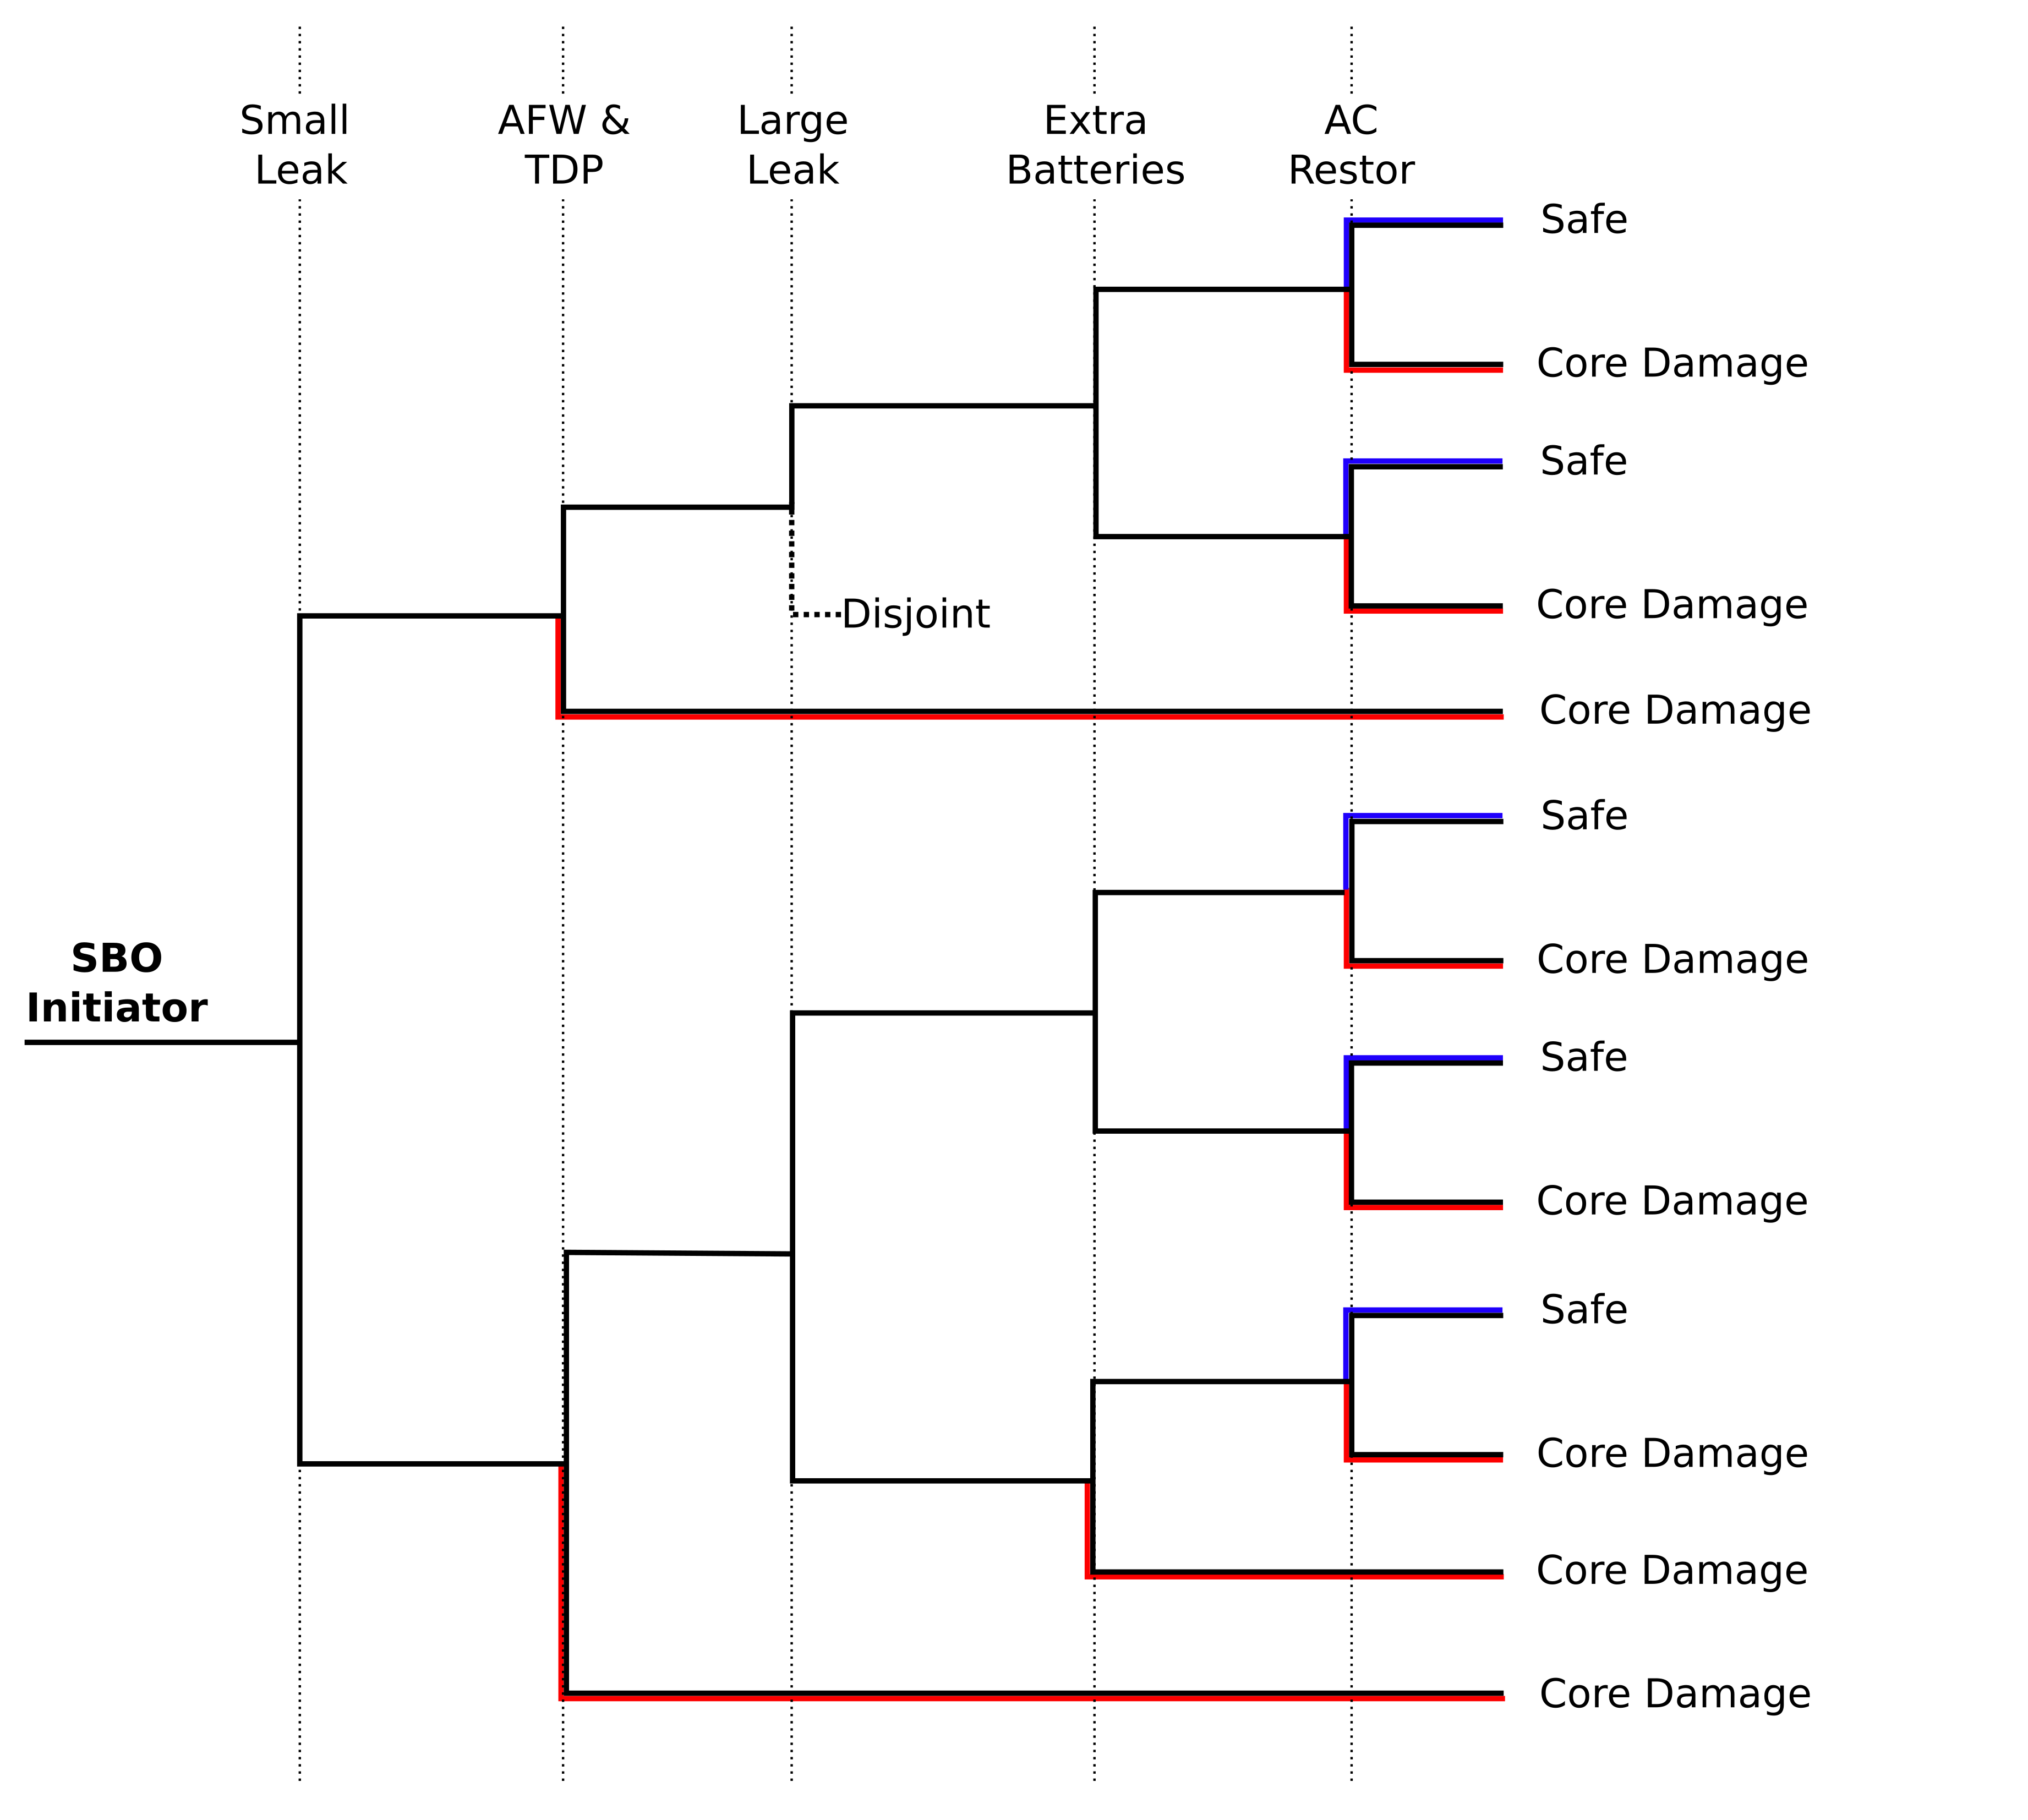
\includegraphics[width=0.55\linewidth]{./Images/sboEventTree.png}
    \caption{\centering Expected Event Tree.}
    \label{fig:event treeeee}
\end{figure}



\subsection{Results}

\begin{table}[H]
\centering
\caption{Results of the simulated sequences: \emph{Y/N} indicates success/failure. Core Damage is obtained when the peak cladding temperatures is higher than 1477K (1204 °C).}
\label{tab:ET_results}
\begin{tabular}{ccccccclr}
\toprule
\textbf{Seq.} & \textbf{TE1} & \textbf{TE2} & \textbf{TE3} & \textbf{TE4} & \textbf{TE5} & \textbf{Outcome} & \textbf{PCT [K]} & $t_\mathrm{CD}$ \textbf{[h]} \\
 & SL & AFW & LL & Batt & AC & & & \\
\midrule
1  & Y & Y & Y & Y & Y & SAFE       & 621  & --- \\
2  & Y & Y & Y & Y & N & CD   & 1702 & 22.52 \\
3  & Y & Y & Y & N & Y & SAFE       & 621  & --- \\
4  & Y & Y & Y & N & N & CD  & 1701 & 18.35 \\
5  & Y & N & Y & Y & Y & SAFE\,$^\dagger$ & 963  & --- \\
6  & N & Y & Y & Y & Y & SAFE       & 621  & --- \\
7  & N & Y & Y & Y & N & CD  & 1701 & 21.19 \\
8  & N & Y & Y & N & Y & SAFE       & 621  & --- \\
9  & N & Y & Y & N & N & CD  & 1701 & 17.39 \\
10 & N & Y & N & Y & Y & SAFE       & 621  & --- \\
11 & N & Y & N & Y & N & CD   & 1701 & 21.32 \\
12 & N & Y & N & N & Y & SAFE       & 621  & --- \\
13 & N & Y & N & N & N & CD  & 1701 & 17.42 \\
14 & N & N & N & Y & Y & CD         & 1478 & 12.21 \\
15 & N & N & N & Y & N & CD  & 1701 & 12.29 \\
\bottomrule
\end{tabular}
\end{table}

\tabref{tab:ET_results} presents the RELAP simulation's results. Several considerations can be made regarding the difference between expected and actual results: 
\begin{itemize}
    \item AC and AFW recovery is the dominant factor that determines whether core damage will occur or not. In all the scenarios when AC and AFW are available, the PCT does not overcome 621 K. The combination of AFW and AC recovery is sufficient to prevent core damage. Once AC power is restored, HPIS and LPIS can keep on cooling the core. 
    \item Sequence 5 (ET5) shows that, even though the AFW is not available, in a condition without leakages through the pump's seal the batteries are able to avoid core damage until the AC power is recovered. This can be explained taking a look at the PCT: without AFW, the temperature rises until the PORV valve starts operating, releasing steam from the pressurizer in order to depressurize the primary. This is different from what we have considered in the preliminary event tree, where the unavailability of AFW determines core damage indipendently from the other systems availability. 
    \item The amplification of the leak, that takes place when the water reaches saturation temperature, has a small effect on the outcome of that sequence. For instance, if we compare ET07 to ET11 or ET09 with ET13, the difference in time is relatively small. This behavior suggest that the main mechanism that lead to core damage is the heat balance through the steam generators, while the leak from the RCP plays a marginal role in the behavior of the plant. 
    \item ET14 can be considered as a "bordeline" case, since its PCT reaches 1478K, slightly above the safety limit. This demonstrates that in presence of leaks from the seals and no AFW, the batteries are not sufficient to prevent core damage. The time needed to reach PCT is 21 minutes higher than the recovery of the AC, which occurs at 12h after the SBO event.  
\end{itemize}

In \figref{fig:event treeeee} all the sequences are plotted, as a function of the peak cladding temperature and the time to reach core damage. 
\begin{figure}[H]
    \centering
    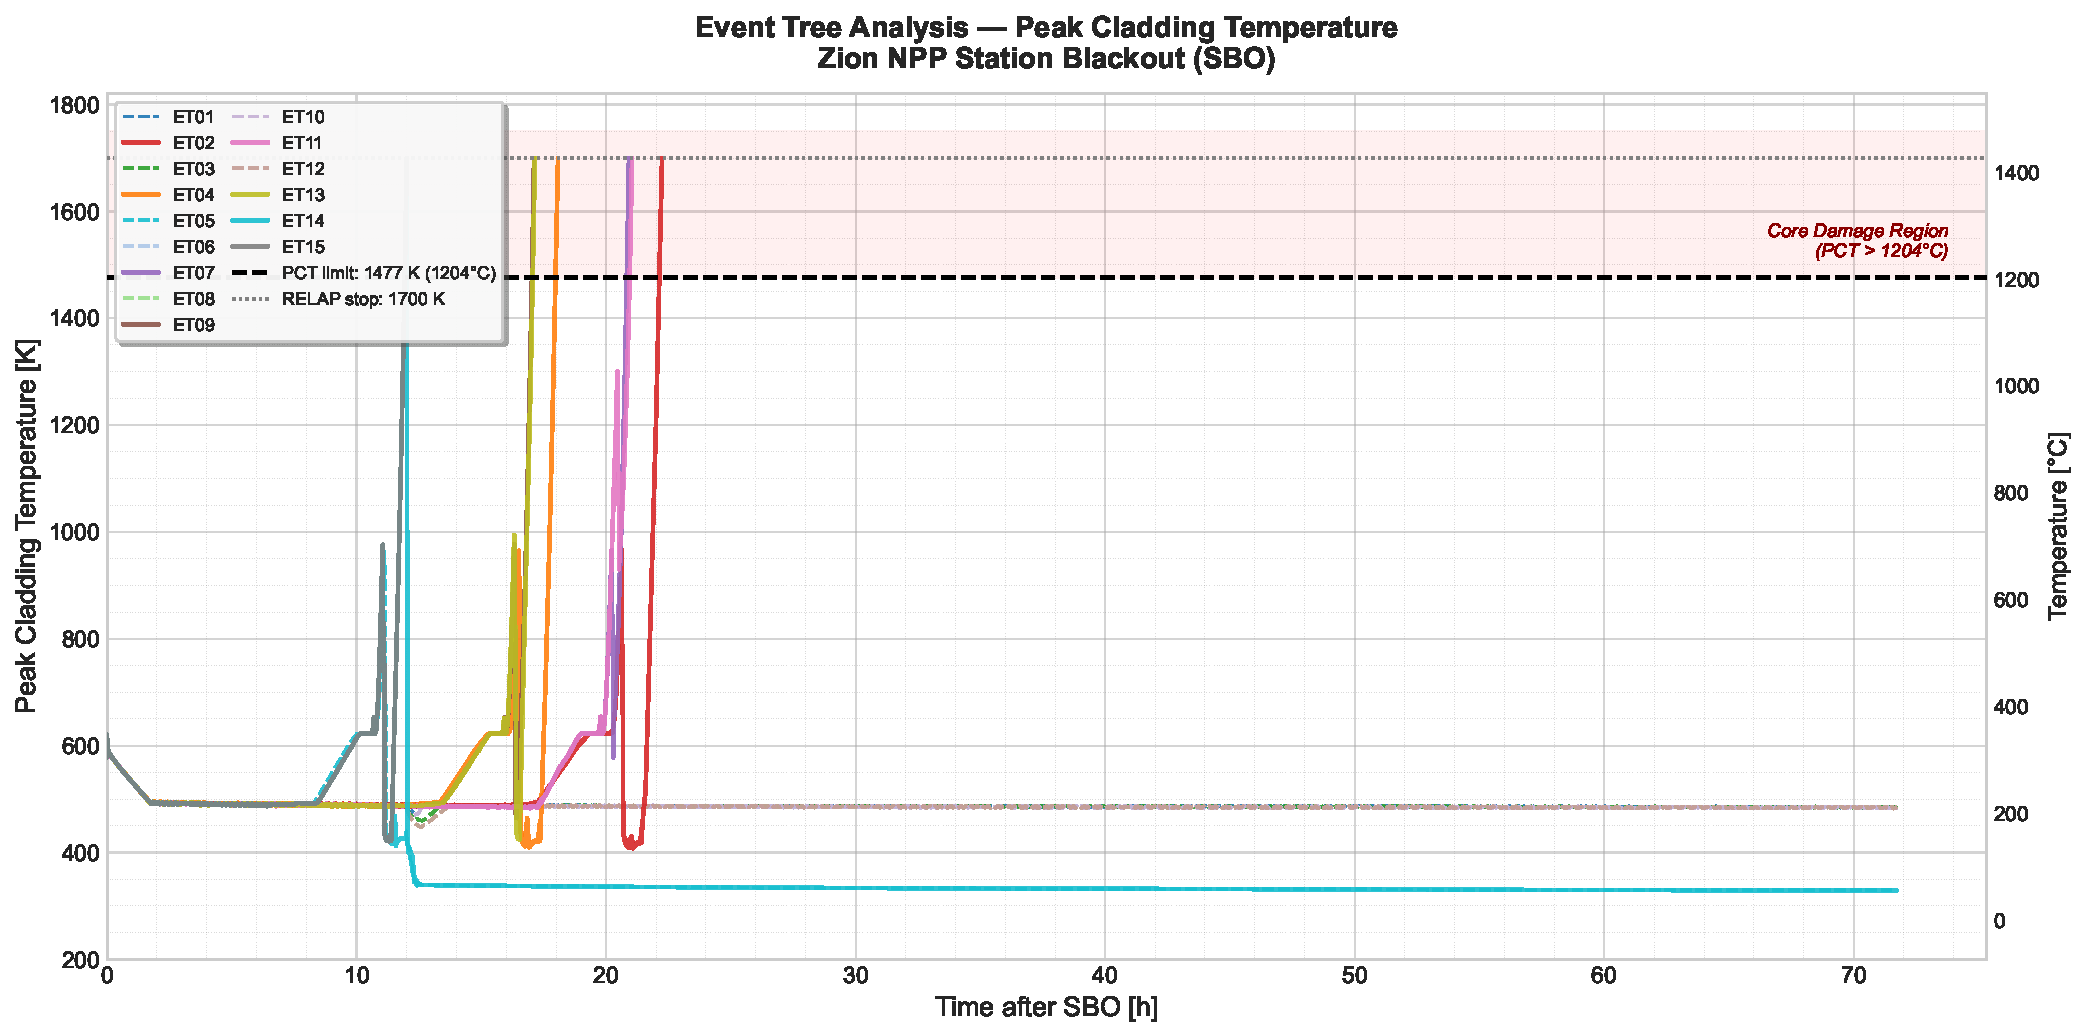
\includegraphics[width=0.75\linewidth]{../Pictures/EventTree/EventTree_PCT_all_cases.pdf}
    \caption{\centering Obtained Event Tree.}
    \label{fig:event treeeee}
\end{figure}

\section{Probabilistic Safety Analysis}

The creation and verification of the event tree for the SBO case allows for the calculation of the contributions of the SBO to the Core Damage Frequency and to identify the Conditional Core Damage Frequency (CCFD).

\subsection{Mathematical Representation}

The first step to analysis the event tree qualitativly is identify the initating event frequency and the conditional probabilities of each of the elements of the event tree. The key variables under consideration are as follows: 

\begin{tabular}{c l}
    $I$ & Initiating Event (SBO)\\
    $LT$ & Long-term SBO\\
    $SB$ & Short-term SBO\\
    $A$ & AFW \& TDP\\
    $S$ & Small Leak\\
    $L$ & Large Leak\\
    $E$ & Extra Batteries \\
    $R$ & Restoration of AC \\
\end{tabular}

In order to calculate the probability of each individual event, first the probability of failure of a single component is calculated. This calculation is followed by a calculation to determine the probability of at least 3 loops working. This is because we consider a conservative approach in our modeling and consider only 3 of our system working. The equation to transform the probability of an individual component failure ($P(F_C)$) to the overall system operability ($P(O)$) is as follows:

\begin{equation}\label{eq:1}
    P(O) = \bigl( \overline{P(F_C)}\bigr)^4 + \bigl(\overline{P(F_C)}\bigr)^3\,P(F_C)\,\bigl(^4_1\bigr)
\end{equation}

\subsubsection*{Initiating Event}

The initiating event frequency of the SBO is derived from the NUREG CR-7110 Vol 2 \cite{nureg7110}. From this report the frequency of Long-Term SBO frequency is identified as $2\text{x}10^{-5}$ pry (per reactor year), and the Short-Term SBO frequency is defined as $2\text{x}10^{-6}$ pry. One interesting finding from this is the higher frequency of long-term SBOs than short term ones. From the frequencies above the initiaing event frequency is derived below:

\begin{flalign}
    F(I) & = F(LT \cup ST) \\ \nonumber
         & = 2 \cdot 10^{-5} + 2 \cdot 10^{-6} \\ \nonumber
         & =  2.2 \cdot 10 ^ {-5} \text{ pry}
\end{flalign}

\subsubsection*{AFW \& TDP}

The AFW and TDP failure frequency is assumed to be largely driven by the failure of the TDP based on the findings of the ORNL CONF-920375-6 analysis \cite{afwFailure}. As such, the probability of failure of this system is taken from the frequency of failure of the TDP system. This system has two failure modes: failure on demand and failure on run. To use a conservative estimate, the sum of the probability of the failure on demand and failure during a mission time of 5 hours is used. The failure on demand probability is:

\begin{equation}
    P(A_d) = 4.6 \cdot 10^{-3} \nonumber
\end{equation}

The failure on run probality is calculated as follows:

\begin{flalign}
    P(A_r) & \approx  \lambda_f \cdot  t_m \\ \nonumber
           &  \approx 8.45 \cdot 10^{-5}  \text{hr}^{-1} \cdot 5 \text{hr} \\ \nonumber
           & \approx 4.225 \cdot 10^{-5} 
\end{flalign}

Giving a total probability of:

\begin{flalign}
    P(A_f) = P(A_d \cup A_r) \\ \nonumber
    P(A_f) = 4.54\text{x}10^{-5}
\end{flalign}

Using equation~\ref{eq:1}, the probability of the operability of the AFW \& TDP is:

\begin{flalign}
    P(A) &= \bigl( \overline{P(A_f)}\bigr)^4 + \bigl(\overline{P(A_f)}\bigr)^3\,P(A_f)\,\bigl(^4_1\bigr) \\ \nonumber
         &=  (1-4.54\text{x}10^{-5})^4 + (1-4.54\text{x}10^{-5})^3 (4.54\text{x}10^{-5}) (4) \\ \nonumber
         &=   0.99999998
\end{flalign}
    

The data for the failure of the TDP was taken from the IHL TDP Performance Analysis \cite{IHL_TDP}.

\subsubsection*{Small Leak}

The small leak event is assumed to happen in the case that the Westinghouse Shut Down Seal fails. A preliminary safety analysis of this component from Westinghouse gives it a conservative failure frequency of 1 in 100 cases giving us the follow probability:

\begin{equation}
    P(S_f) = 0.01 \nonumber
\end{equation}

This leads to an operability probability of:

\begin{equation}
    P(S) = 0.99940 \nonumber
\end{equation}

\subsubsection*{Large Leak}

Large leaks in the RCP seals occur in the situation in which saturation temperatures are reached. The conditional probability of this event during an SBO is listed in the NUREG CR-7110 Vol. 2 report \cite{nureg7110}, it gives a the following conditional proability. 

\begin{equation}
    P(L_f) = 0.2 \nonumber
\end{equation}

For the overall operability of the large leak condition, it is assumed that the system fails even if there only a single large leak in a pump. This gives the following proability:

\begin{flalign}
    P(L) &= \biggl( 1-P(L_f) \biggr)^4 \\ \nonumber
        &= 0.4096
\end{flalign}

The conditional probability is used in this case as the probability of a large leak dramatically increases during an SBO event. 

\subsubsection*{Extra Batteries}

This section was the most difficult to model. This is because the existence of additional batteries is either an existing plant aspect or the result of proper load shedding which requires extensive human error analysis. In the end, the probability of the extra batteries has a long impact on the overall CCDP as seen in Equation~/ref{eq:CCDP} below. An alternative method to determine this probability is considering the proper implementation of FLEX-DG (portable diesel generators) that are now implemented in all US NPP and the vast majority of the global fleet.

The analysis of the proper operator installation and equipment performance is done in Universidad Politíecnica de Madrid \cite{flex}. This gives the follow probability below where $P(E_o)$ and $P(E_f)$ are the probabilities of operator human error and the probability of equipment functionality respectively:

\begin{flalign}
    P(E) & = \overline{P(E_o)} + \overline{P(E_f)} \\ \nonumber
         & =  0.015 + 0.2905 \\ \nonumber
         & =  0.3055
\end{flalign}

\subsubsection*{AC Power Restoration}

The AC power restoration after 12 hours is estimating using the conditional probability of a long term SBO given an SBO event. This method allows us to obtain the probability that AC power is restored within a 12-hour window. The calculation is done using Bayes Theorem for conditional probabilities:

\begin{flalign}
    P(R_f)    & = P(LT|I) \\ \nonumber
            & =\frac{P(I|LT)*P(LT)}{P(I)} \\ \nonumber
            & = \frac{1(2\text{x}10^{-5})}{2.2\text{x}10^{-5}} \\ \nonumber
            & = 0.909
\end{flalign}

Similarly to the large leak condition, the Restore AC probability is not subject to equation~\ref{eq:1}. This is because the Bayesian analysis above is down for at plant level and not at an individual component level. So the probability of success is:
\begin{equation}
    P(R) = 0.091 \nonumber
\end{equation}


\subsection{CCDP}

The conditional core damage frequency is the probability of core damage given an initiating event happens. This allows for the analysis of the consequence of an event even if the event is exceedingly rare. To begin the analysis, a boolean representation of the event tree is made using the sum of the Minimal Cut Sets followed by the simplification of the equation. The minimum cut sets are the paths that lead to core damage and are taken from \figref{fig:event treeeee}. The equation begins as follows:

\begin{flalign}
    P(CD|I) = & \; P(S)\, P(A)\, P(E)\, \overline{P(R)}  \\ \nonumber
              & + P(S)\, P(A)\, \overline{P(E)}\, \overline{P(R)}  \\ \nonumber
              & + P(S)\, \overline{P(A)} \\ \nonumber
              & + \overline{P(S)}\, P(A)\, P(L)\, P(E)\, \overline{P(R)}  \\ \nonumber
              & + \overline{P(S)}\, P(A)\, P(L)\, \overline{P(E)}\, \overline{P(R)}  \\ \nonumber
              & + \overline{P(S)}\, P(A)\, \overline{P(L)}\, P(E)\, \overline{P(R)}  \\ \nonumber
              & + \overline{P(S)}\, P(A)\, \overline{P(L)}\, \overline{P(E)} \\ \nonumber
              & + \overline{P(S)}\, \overline{P(A)}
\end{flalign}

This equation is then simplified using boolean algebra identifies to get the final CCDP equation below:

\begin{flalign}\label{eq:CCDP}
    P(CD|I) = & \; \overline{P(A)} + P(S)P(A)\overline{P(R)}+  \biggl( \overline{P(E)}+P(E)\overline{P(R)}   \biggr)  \biggl( \overline{P(S)}P(A)\overline{P(L)} \biggr)  \\ \nonumber
            = &\; 1.2\text{x}10^{-8} + 0.908 + (0.1928)(0.00035) \\ \nonumber
            = & \; 0.908
\end{flalign}

\subsection{Core Damage Frequency}

\begin{flalign}
    F(CD) & = F(I)\;P(CD|I) \\ \nonumber
          & = (2,2\cdot10^{-5})(0.908)\\ \nonumber
          & = 1.99\cdot10^{-5}
\end{flalign}

This number is incredibly high in terms of plant safety. However, this is incredibly similar to analyzes down by the NRC, in for the Surry NPP \cite{Surry}, the total core damage frequency from all SBO initiating events (SBO+Battery Depletion, SBO+SBLOCA, SBO+AFWfail + SBO+SORV + ...) is $2.7664\cdot10^{-5}$ pry. This puts the above estimate well within the same order of magnitude. The core damage frequency for the Zion NPP is a similar estimate of $9.34\cdot10^{-6}$ from the NRC \cite{ZionCD}. 

\section{Safety System Implementation: Passive Secondary Heat Removal System}
\label{sec:pshrs}

The Passive Secondary Heat Removal System (PSHRS) has been designed to extend
the SBO coping capability of the Zion NPP from the current 12~h up to the
72~h required by the revised 10~CFR~50.63. The system is fully passive:
it does not rely on AC power, AAC sources, active pumps, compressed air,
or operator action once the actuation condition is reached.

The PSHRS consists of a closed natural-circulation loop connected in
parallel to the Main Steam Line (MSL) and the Main Feedwater Line of each
Steam Generator, with all connections placed \emph{outside} the containment
in order to avoid additional containment penetrations (GDC~54). The loop
routes saturated steam from the SG outlet to a vertical tube-bundle Heat
Exchanger (HX) immersed in an Elevated Evaporation Pool (EEP) located
above the SG elevation. The steam condenses on the HX tubes, and the
condensate returns by gravity to the SG feedwater line, closing the loop.
The heat absorbed by the pool is removed by evaporation to the atmosphere
through a dedicated vent line at the top of the EEP enclosure. The driving
head is provided by the density difference between the saturated vapour
in the hot leg and the subcooled condensate in the cold leg, both at the
secondary-side pressure of $\sim$67~bar.

Isolation during normal plant operation is ensured by fail-open
electromagnetic valves arranged in a series--parallel configuration that
satisfies the single failure criterion: valves required to open on demand
are placed in parallel, while valves required to remain closed during
power operation are placed in series. The system is normally kept closed
by the DC bus; upon sustained loss of both AC and DC power
(filtered to discriminate the short transient at battery switch-over),
the valves automatically open and natural circulation establishes itself.

The peak thermal load on the system occurs at $t = 5$~h after SBO, when
the DC batteries are depleted and the AFW Turbine-Driven Pump becomes
uncontrolled. This instant defines the worst-case condition for the
hydraulic sizing of the loop. The main design parameters are summarised
in Table~\ref{tab:pshrs_design}.

\begin{table}[H]
\centering
\caption{Main design parameters of the PSHRS (per loop).}
\label{tab:pshrs_design}
\begin{tabular}{lcc}
\hline
Parameter & Value & Unit \\
\hline
Reactor thermal power $P_0$              & 3250                  & MW$_{\text{th}}$ \\
Peak decay power at $t=5$\,h             & 31.8                  & MW \\
Total decay energy ($5$--$72$\,h)        & $4.286\times10^{12}$  & J \\
Secondary-side pressure                  & 67                    & bar \\
Latent heat of vaporisation at 67\,bar   & 1524                  & kJ/kg \\
Saturated liquid density at 67\,bar      & 745.28                & kg/m$^{3}$ \\
Saturated vapour density at 67\,bar      & 34.786                & kg/m$^{3}$ \\
Required steam mass flow rate per loop   & 5.22                  & kg/s \\
Elevation difference $H$ (SG--HX)        & 8.5                   & m \\
Natural circulation driving pressure     & $5.92\times10^{4}$    & Pa \\
Minimum pipe diameter $D_{\min}$         & 0.125                 & m \\
Steam velocity at $D_{\min}$             & 12.16                 & m/s \\
Reynolds number at $D_{\min}$            & $2.65\times10^{6}$    & -- \\
Total pressure losses                    & $5.48\times10^{4}$    & Pa \\
Natural circulation margin               & 1.08                  & -- \\
Evaporated water mass (5--72\,h)         & 1652.9                & t \\
Required pool volume (incl.\ 20\% margin)& 1989.5                & m$^{3}$ \\
\hline
\end{tabular}
\end{table}

The natural-circulation margin $\Delta p_{\text{drive}}/\Delta p_{\text{loss}}=1.08$
confirms that the loop is self-driven under worst-case conditions,
while the pool inventory is sufficient to absorb the decay energy
released between battery depletion and AC restoration at $t=72$\,h.



\subsection{Design Modifications from the Preliminary Configuration}
\label{sec:pshrs_mods}

With respect to the preliminary design presented in the hydraulic
pre-sizing report, three modifications have been introduced in order to
improve the robustness of the system, simplify its actuation logic and
guarantee the integrity of the natural-circulation flow path during the
entire 72-hour transient.

\paragraph{T-shaped Evaporation Pool.}
The EEP has been reshaped from a uniform prismatic geometry to a
T-shaped cross-section, with a wider upper section acting as the main
evaporation reservoir and a narrower lower section that hosts the Heat
Exchanger bundle. This geometry guarantees that the HX remains fully
submerged throughout the transient even after a significant fraction of
the pool inventory has been boiled off: as the pool level decreases
with time, the residual water remains confined in the narrow lower
section, preserving the heat transfer surface in contact with liquid
water. In the original cylindrical/prismatic design, the same loss of
inventory would have produced a faster drop in water level and a
premature partial uncovery of the HX tubes, degrading the condensation
performance well before the 72-h mission time. The total water inventory
is unchanged with respect to the value reported in
Table~\ref{tab:pshrs_design}, but its vertical distribution is now
optimised to maintain HX submergence as the dominant geometric
constraint.

\paragraph{Enlarged Atmospheric Vent.}
The cross-sectional area of the vent line connecting the EEP headspace
to the atmosphere has been increased with respect to the preliminary
sizing. The objective is to keep the pool effectively at atmospheric
pressure during the entire transient, avoiding pressurisation of the
EEP enclosure caused by the steam generated by pool boiling.
A pressurised pool would raise the saturation temperature of the water,
reduce the temperature difference available for condensation on the HX
tubes and ultimately reduce the heat removal capability of the system.
The enlarged vent ensures that the steam produced at the peak
evaporation rate can be discharged without appreciable pressure
build-up, keeping the pool boundary condition consistent with the
hypothesis used in the sizing calculations
($p_{\text{pool}} \approx p_{\text{atm}}$, $T_{\text{sat}} \approx 100^{\circ}$C).

\paragraph{Delayed Actuation (5\,h after SBO).}
The actuation logic has been tied to the depletion of the DC batteries
at $t \approx 5$\,h after the initiating event, rather than to the SBO
signal itself. During the first 5\,h, decay heat removal is already
ensured by the existing Turbine-Driven AFW supplied from the
Condensate Storage Tank and controlled through DC power. Activating
the PSHRS during this phase would be redundant and could interfere
with AFW operation, introduce unnecessary pool inventory consumption
and complicate the cooldown strategy followed by the operators.
The PSHRS is therefore designed to engage exactly when the existing
heat-removal chain is about to be lost: the fail-open isolation valves
open upon sustained loss of the DC signal, with a time-filter that
discriminates the brief AC-to-DC switch-over from a genuine battery
depletion. This staged actuation maximises the useful pool inventory
available for the long-term passive phase and ensures a smooth
hand-over from the active (AFW + batteries) to the passive (PSHRS)
heat removal mode.





\section{Conclusions}

The steady-state calculation is first checked against the target values, and the SBO base case is then used to observe the main thermal-hydraulic response of the plant under blackout conditions. \\

The SBO base case transient showed that the plant is able to maintain core cooling for at least 12 hours without core damage. The decay heat is effectively removed through natural circulation in the primary system and by the Auxiliary Feedwater system on the secondary side. The peak cladding temperature remains well below the safety limit of 1477 K throughout the entire transient, and the core is never uncovered. 

Having analyzed two EOPs, we can say that the SG cooldown procedure (EOP 1) proved usefil but not strictly necessary to prevent core damage within the 12-hour simulation window. The cooldown EOP reduces primary pressure and lowers the RCP seal leak rate. It is therefore recommended as a prudent operator action. Instead, the primary depressurization procedure (EOP 2) was never triggered in either the base case or the no-cooldown case, as the Core Exit Temperature did not reach the 923 K threshold at any point during the transient. 
Overall, the results demonstrate that the existing safety systems and operator procedures are sufficient to manage the SBO scenario for 12 hours. However, the analysis also highlights that the absence of the SG cooldown EOP leads to a more challenging scenario and could lead to core damage in a longer event. \\

The event tree proved that the AC power restoration is the most relevant action in order to avoid core damage in most of the cases analyzed. In every related case, the PCT stays below the safety limit for core damage and the outcome is safe regardless of the seal leak, its amplification or extra-batteries availability. AC restoration is therefore the most important risk reduction factor. Moreover, seal leak amplification has a marginal impact on the system condition. Comparison between cases where the TE3 is present (i.e. ET07 vs ET11, or ET09 vs ET13)shows that the difference in time to core damage is at most 2 hours and the asymptotic PCT is almost identical. This confirm that, in the time scale considered for this scenario, the dominant mechanism of failure is the loss of heat sink rather than the loss of inventory from the RCP seals. 

\newpage

\section*{CRediT Author Statement}

\begin{itemize}
    \item \textbf{Filippo Dalmonego:} Coding, Writing, Review, Supervision, Visualization.
    \item \textbf{Tyler Ewald:} Coding, Writing, Editing, Supervision.
    \item \textbf{Riccardo Fasano:} Writing, Coding, Editing, Supervision.
    \item \textbf{Francesco Qualizza:} Methodology, Supervision, Writing, Editing.
\end{itemize}

\printbibliography
\end{document}
